
%--------------------------------------------------------------------------
% THESIS: The MAIN thesis file from which all other things are included.
%--------------------------------------------------------------------------

% Include the header which includes packages, the Acadia style and definitions.

%---------------------------------------------------------
% Header: This file includes all the packages and custom definitions
% we have used in this example thesis.
%----------------------------------------------------------

% Uncomment the following line if, for some reason, you want a PDF 1.4
% document, rather than (at time of writing) PDF 1.5.
% \pdfminorversion=4

\documentclass[12pt,twoside,openright]{report}

%---------------------
% START: Packages
%---------------------
\usepackage{textcomp}
\usepackage[latin1]{inputenc}
\usepackage{amsmath}
\usepackage{amsfonts}
\usepackage{amssymb}
\usepackage{amsthm}
\usepackage{graphicx}
\usepackage{soul}
\usepackage{listings}
\usepackage{subfig}
\usepackage{verbatim}
\usepackage{alltt}

% There are used in the graphics chapter.
% You can delete the following two lines if you use no tikz/pgf graphics
% in your thesis.
\usepackage{tikz}
\usepackage{pgfplots}

% Load the natbib citation package: set the citations to be numerical
% with square brackets separated by commas.
\usepackage[numbers,square,comma]{natbib}

% Now include the Acadia thesis style
\usepackage{acadia-hon-thesis}

% Load the hyperref package.
% The options tell it to (a) use hyper-links to pages with Roman
% numerals that are different than pages with Arabic numbers, and
% (b) tell Adobe reader to show a page number matching the thesis page
% number (rather than sequentially numbering the PDF pages from 1).
\usepackage[plainpages=false,pdfpagelabels]{hyperref}

% The information in the first three lines here goes into the PDF
% document properties.
% The rest of the lines define options related to hyper-links.
% colorlinks: typeset links in the given colours
%	      (otherwise an ugly box is drawn around the links, although
%	       it is only seen on the screen, not in printed copies)
% A newer option (since May 2011) would be to just use the hidelinks option.
% Note: pdfprintscaling=None should discourage Adobe reader from wanting to
% scale your pages to fit printable area when you print from Adobe reader.
\hypersetup{%
    pdftitle={PUT YOUR THESIS TITLE HERE},
    pdfauthor={PUT YOUR NAME HERE},
    pdfkeywords={PUT ANY KEYWORDS HERE},
    colorlinks = true,
    linkcolor = black,
    anchorcolor = black,
    citecolor = black,
    filecolor = black,
    urlcolor = black,
    pdfprintscaling=None
}


% Load the algorithm/mic packages and use chapter-wise numbering
\usepackage[chapter]{algorithm}
\usepackage{algorithmic}


% JD addition:
% The url package does not, by default, allow breaks at '-'.  Change this
% by adding \do\- to this macro.  If you don't want breaks at '-' in URLs,
% just comment out or delete these lines:
\def\UrlBreaks{\do\.\do\@\do\\\do\/\do\!\do\_\do\|\do\;\do\>\do\]\do\-%
               \do\)\do\,\do\?\do\'\do+\do\=\do\#}%


%---------------------
% END: Packages
%---------------------
\bibliographystyle{plainnat}

% The depth of the table of contents: change the MAXIMUM depth of
% citations in your table of contents.
\setcounter{tocdepth}{6}

%
% Some definitions of commands used in this thesis
%

% For instance, if you have an acronym you like to use, then define a
% command, it's faster and if the acronym changes you only have to
% change it in one place.
\def\sysacro{SPECIALACRONYM}

% Allow us to change the margins easily and at will
\newenvironment{changemargin}[2]{%
  \begin{list}{}{%
    \setlength{\topsep}{0pt}%
    \setlength{\leftmargin}{#1}%
    \setlength{\rightmargin}{#2}%
    \setlength{\listparindent}{\parindent}%
    \setlength{\itemindent}{\parindent}%
    \setlength{\parsep}{\parskip}%
  }%
  \item[]}{\end{list}}

%setup the default format of listings
\lstset{
    basicstyle=\footnotesize,
    numbers=left,
    xleftmargin=5mm,
    linewidth=\textwidth,
    breaklines,
    frame=tb,
    frameround=fttt
}

% A new definition style
\newtheoremstyle{defstyle}	% name
    {3pt}			% Space above
    {3pt}			% Space below
    {}				% Body font
    {}				% Indent amount
    {\itshape}			% Theorem head font
    {:}				% Punctuation after theorem head
    {.5em}			% Space after theorem head
    {}		% Theorem head spec (can be left empty,meaning 'normal�)
\theoremstyle{definition}
\newtheorem{definition}{Definition}[chapter]


% Change comment style for algorithms
\renewcommand{\algorithmiccomment}[1]{/*#1*/}
% Change Require: to Input: for algorithms
\renewcommand{\algorithmicrequire}{\textbf{Input:}}
% Change Ensure: to Output: for algorithms
\renewcommand{\algorithmicensure}{\textbf{Output:}}


\begin{document}
    %% START NOTE: In your real thesis, DO NOT include these lines.
    %% Using your text editor, delete all the lines from ``START NOTE''
    %% just above to ``END OF START NOTE'' way down below.
    \begin{center}
	DO NOT INCLUDE THESE PAGES IN YOUR THESIS! THIS IS FOR
	INSTRUCTION ONLY! 
    \end{center}
    \small
    The main file for this thesis is \verb|thesis.tex|.  All other
    files are \verb|include|d from \verb|thesis.tex| or another
    \verb|include|d file!
	
    The \verb|.tex| files used in this example thesis are:
    \begin{itemize}
	\item \verb|thesis.tex|: The main thesis file from which
	    everything is included. 
	\item \verb|header.tex|: Includes the packages, styles, and
	    definitions used in this example. 
	\item \verb|algorithms-and-listings.tex|: Included from
	    \verb|thesis.tex| --- Examples of typesetting algorithms and code
	    listings. 
	\item \verb|citations.tex|: Included from \verb|thesis.tex| ---
	    Examples of citations using \LaTeX's \verb|natbib| package. 
	\item \verb|figures-and-tables.tex|: Included from
	    \verb|thesis.tex| --- Examples of figures, tables and sub-floats. 
	\item \verb|fine-points.tex|: Included from \verb|thesis.tex| --- 
	    Some fine points of typesetting, to give your thesis even
	    more of a polished touch.
	\item \verb|formatting.tex|: Included from
	    \verb|thesis.tex| --- Examples of formatting and spacing issues. 
	\item \verb|getting-started.tex|: Included from
	    \verb|thesis.tex| --- A few notes on how to get started
	    using \LaTeX\ according to your chosen operating system.
	\item \verb|graphics-info.tex|: Included from
	    \verb|thesis.tex| --- Information about including graphics
		in your thesis.
	\item \verb|introduction.tex|: Included from \verb|thesis.tex|
	    --- A short introduction.
	\item \verb|lists.tex|: Included from \verb|thesis.tex| ---
	    Information about how you create lists of things.
	\item \verb|packages.tex|: Included from \verb|thesis.tex| ---
	    Describes the various packages used in this example. 
	\item \verb|preliminaries.tex|: Included from
	    \verb|thesis.tex| --- The file from which the thesis
	    template draws personal details about the thesis
	    (e.g., thesis title, you name, your advisor, etc.).
	\item \verb|sections.tex|: Included from \verb|thesis.tex| ---
	    How to use the sectioning features of \LaTeX.
	\item \verb|websites.tex|: Included from \verb|thesis.tex| --- A
	    few web sites that you may find useful.
    \end{itemize}
	
    \begin{center}
	DO NOT INCLUDE THESE PAGES IN YOUR THESIS! THIS IS FOR
	INSTRUCTION ONLY!
    \end{center}

    \vfill
    \noindent
    This document was last updated April 28, 2015.
	
    %% END OF START NOTE: INCLUDE THE REST!

    % PRELIMINARIES: This is the file you will use to setup your
    % name, date, advisor, etc. 
    %---------------------------------------------------------
% Preliminaries: Set up your own details in this file!
%----------------------------------------------------------

% Don't forget to remove the ()s in ALL of these "personalization" lines.

\title{(PUT YOUR THESIS TITLE IN preliminaries.tex)}
\author{(PUT YOUR FULL NAME IN preliminaries.tex)}
\dept{(PUT YOUR DEPT IN preliminaries.tex)}   % E.g., Physics, Computer Science,
\deptOrSchool{(Department or School)}         % Pick one, remove the rest
\degree{(PUT YOUR DEGREE IN preliminaries.tex)}  % E.g., Science, Arts, ...

\submissionMonth{(March)}	    % OR WHATEVER MONTH YOU ACTUALLY SUBMIT IN
\submissionYear{(20XX)}
\copyrightYear{(20XX)}		    % Probably the same as submissionYear.

% Use a "~" after the "r." of "Dr." so that TeX doesn't think you have
% ended a sentence (at which point it gives extra space).
\supervisor{(Dr.~Your Supervisor)}

% Remove the '%' from the next line and fill in the name if desired.
%\cosupervisor{(Dr.~Your Other Supervisor)}

\headOrDirector{(Dr.~The Head or Director)}
% If the head or director is an ``acting'' head or director, uncomment
% the next line (i.e., delete the '%'):
% \justActing

% You will have to ask around to find out the name of the person
% to put here... it changes from year to year.
\honoursCommittee{(The honours committee person)}

%-------------------------------------------------------------------------

% This outputs the title page, the approval page and the copyright page.
\firstThreePages

%-------------------------------------------------------------------------
% Now write your acknowledgements (if any).
% If you wish to acknowledge no-one, delete or comment-out the
% next few lines.

\Acknowledgments

Place any acknowledgments you might want to make here.

Don't forget to be formal and professional.

%-------------------------------------------------------------------------

% This outputs the table of contents, lists of figures, tables, ...

\tocAndSuch

%-------------------------------------------------------------------------

\prefacesection{Abstract}

This is a ``quick-start'' guide to help you use \LaTeX\ to produce
your thesis.  It by no means covers all issues, but it should give you
a solid start.

\TeX\ is a system developed by Donald Knuth with the goal of doing
beautiful typesetting, particularly for documents which use
mathematics.  It is one of the first significant programs made
available to the world at large \emph{for free} by its author.  By
design, Knuth has dictated that \TeX\ won't change any more, which
means that \TeX\ documents won't become unusable because of
incompatible updates.  (However, other people are extending \TeX, so
it is not a ``dead'' system.)

\LaTeX\ is a set of additions to \TeX\ which arguably make it easier
to produce documents.  This sample thesis will assume you are going to
use \LaTeX\, but if you later to decide to try Knuth's ``plain'' \TeX,
you will find that the concepts are fairly similar.

This document was initially written by Brian Demmings; any ``I'' found
in this document refers to Brian.  Jim Diamond has updated it
occasionally since Brian graduated, and hopes he has only improved
things with his changes.  Alex Sanford took the masters template and
transmogrified it into the honours thesis template.

The ``source code'' of this document should be in the same directory
as the nicely-formatted PDF file you are reading.  If you want to see
exactly how anything here is produced, just look in the appropriate
``source code'' file.  (For example\dots\ if you read the source code,
you will see that we used ``\verb|\dots|'' rather than ``\verb|...|'',
since the spacing of ``\dots'' is better than ``...''.)

\medskip

Write \emph{your} abstract here (in the file \verb|preliminaries.tex|).
		
\medskip

\textbf{BEWARE:} Some of the techniques (e.g., the ``Table of
Algorithms/Listings'') may \emph{not} be permitted.  When in doubt
check with RGS (masters students), the registrar (honours students) or
your advisor.


%-------------------------------------------------------------------------

% Don't mess with this line!
\afterpreface


    % CHAPTER CONTENT START
    % Replace all the lines from here down to ``CHAPTER CONTENT END''
    % with a collection of ``\include{XYZ}'' lines, where each such XYZ
    % is the name of a text file holding (for example) one chapter of
    % your thesis.
    % If you have appendices you need that ``\appendix'' line BEFORE
    % you \include your appendices.
    \chapter{Getting Started}

The basic idea of \LaTeX\ (and ``plain'' \TeX) is that you create one
or more \emph{plain text} ``source files'' using any text editor (but
not word processor!\null) of your choice, and then ``compile'' your
source files into a nicely-formatted document (normally a PDF file).
This work flow separates the writing of your ideas from the formatting
and style details, allowing you to concentrate on what you want to
say, without simultaneously worrying about getting the look ``just
so''.  In particular, this thesis template allows you to create a
document meeting Acadia's thesis formatting requirements without
having to worry about all the details of the front pages, page
numbering, lists of figures and tables, and so on\dots\ it just
happens automatically for you.  But, if some time later you wish to
publish your writing elsewhere (e.g., a journal or conference), you
can change the few lines which specify the formatting, select the
parts of your work you want to publish, and re-compile.

To use \LaTeX\ (or plain \TeX) to produce your thesis (or other
documents or presentations) you need to have a \TeX\ ``distribution''
installed on your computer, or you need to have a so-called ``live
\TeX\ DVD''.  The former is preferable to the latter, unless you are
extremely short of disk space.

As mentioned in the abstract, and given the existence of this thesis
template, the quickest way to get going with the \TeX\ system is to
use the \LaTeX\ package.  \LaTeX\ can be used to create so-called
``\verb|.dvi|'' files, from which you can subsequently create
PostScript or Adobe PDF files.  However, \LaTeX\ can also directly
create PDF files, and this route is strongly recommended for the most
users.  (There are two reasons for this recommendation.  First, since
the library wants a PDF file, there are less steps involved if you
just create a PDF file from the get-go.  Second, it is easier to
include \emph{most} graphics made with other programs (photographs,
plots, \dots) using the ``flavour'' of \LaTeX\ which creates PDF
files.)

You can download (for free!\null) a \TeX\ distribution from
\url{http://www.tug.org/texlive/} for many different systems.
However, if your operating system supplier provides an up-to-date
\TeX\ distribution, you may (or may not!\null) find it easier to just
use that.  The way you use \LaTeX\ varies a bit, depending on which
operating system you use on your computer, as well as which
\TeX\ system you installed on your computer.  The next three
subsections give some operating system-specific details.

You can use an ordinary text editor to create or edit your ``source
files'', but there are some editors which are specifically designed
for creating \TeX\ or \LaTeX\ documents.  Three such editors, all
available for free, are
\begin{itemize} \itemsep0pt
\item \TeX{}studio, available at
\url{http://texstudio.sourceforge.net/},
\item Texmaker,
available at \url{http://www.xm1math.net/texmaker/}, and
\item \TeX{}works, available at \url{http://www.tug.org/texworks/}.
\end{itemize}
A comparison of these (and others) can be found at
\url{http://en.wikipedia.org/wiki/Comparison_of_TeX_editors}.

\section{Using Linux}

% If, when you read this, there is once again an Acadia Linux template, it
% might come with \TeX\ and \LaTeX\ installed.  If you use some other
% distribution of Linux, you should be able to download and install one
% or more packages to get it running on your system.

Regardless of which Linux distribution you use, you should be able to
download and install one or more packages to get \TeX\ and
\LaTeX\ running on your system (if the \TeX\ system is not already
installed).  Look through the list of packages available for download
and installation for your distribution.  For example, in Ubuntu-type
systems you can use your GUI package manager to install the \verb|tex|
package, or from the command line you can type
``\verb|sudo apt-get install tex|''.  This is a big download; make
sure your network connection is good and you have more than a minute
or two for the download to complete.

If you are unable to find anything, the \TeX\ Live distribution is
fairly easy to install; the instructions are found at the web site
given above.

\TeX{}live for Linux does not provide (what a computer scientists
might call) an integrated development environment (IDE), but some
people like the combination of \verb|emacs| and \verb|auctex|.
Alternatively, you might like to try out one of the free \TeX\ editors
mentioned above.  However, the command-line usage of \LaTeX\ is very
straightforward, so you might decide that you don't need to spend time
trying to find a suitable IDE.

To compile any \LaTeX\ document from the command line, you can either
use the program \verb|latex|, which produces ``\verb|.dvi|'' files, or
you can use \verb|pdflatex|, which produces ``\verb|.pdf|'' files.
All things being equal, the latter is probably the best choice.  Of
course, most people (as well as the library) will be able to use a PDF
file, but if you produce a \verb|.dvi| file, you will need to use a
post-processor to create a PDF or PostScript file.  The \verb|.dvi|
approach is probably only of interest to you if you want to use the
power of the PostScript language to do tricky things.

Having created one or more \LaTeX\ source files using your favourite
text editor, the next step is to ``compile'' your document into a
PDF file.  This can be done with the following steps.  First,
assuming that your document is in a file called \verb|thesis.tex| (or
that \verb|thesis.tex| includes all of the files comprising your
document), run

\verb|pdflatex thesis.tex|

\noindent
Note that under Linux you do not need to type the ``\verb|.tex|'',
\verb|pdflatex| will add that for free.  Assuming you are using
\verb|bibtex| to process your citations, next run

\verb|bibtex thesis|

\noindent
Finally, to ensure that all of the references in your document are
correct, re-run \verb|pdflatex| twice (yes, twice):

\verb|pdflatex thesis|

\noindent
You can, of course, type all these on one line, as follows:

\verb|pdflatex thesis && bibtex thesis && pdflatex thesis && pdflatex thesis|

\noindent
If for some reason you want to go the \verb|.dvi| route, use
\verb|latex| instead of \verb|pdflatex| in the examples above.
Then, you can create a PostScript file by running

\verb|dvips thesis.dvi -o thesis.ps|

\noindent
and if you want to create a PDF file from that you can run the
command

\verb|ps2pdf thesis.ps|

\noindent
Alternatively, a PDF file can be created directly from the \verb|.dvi|
file with the command

\verb|dvipdfm thesis.dvi|

\smallskip
There is a ``\verb|Makefile|'' in the thesis template directory with
the other files.  You can just type \verb|make| to create a new PDF
version of your thesis whenever you have made some changes.  The
Makefile is a bit heavy-handed, since it runs \verb|pdflatex| three
times and \verb|bibtex| once, even if one run of \verb|pdflatex| would
suffice.  Ho hum.

\section{Using MS Windows}

\subsection{IDE}
A (MS Windows-only) IDE which many people use to write \LaTeX\ is
called TeXnic Center; at time of writing it can be found at:
\url{http://www.texniccenter.org/}.

You can use any text editor to edit \verb|.tex| files, but TeXnic Center
provides useful extras.
Another alternative, \verb|Texmaker|, which is also available for
Linux and OS X, can be found at \url{http://www.xm1math.net/texmaker/}.

\subsection{Support in MS-Windows}

TeXnic Center relies on MiKTex to perform the actual compiling
into DVI, PS, PDF, etc.  MiKTex can be found at
\url{http://www.miktex.org/}.
You'll need to install MiKTex \emph{before} installing TeXnic Center.

\subsection{Command Line Support}

You may choose to type commands in to a command window, rather than
using the pointy-clicky features of TeXnic Center or \verb|Texmaker|.
The next subsection describes how to do that.  But if you like the
pointy-clicky method, you can skip the rest of this subsection.

\subsubsection{Option 1: \emph{pdflatex}}

To compile a \verb|.tex| document that uses citations in \verb|bibtex|
format (see Section~\ref{sec:CITATIONS}) we must compile the document
in a specific order.  For example, using the \verb|thesis.tex| file in
used to produce this document:

First run:

\verb|pdflatex -interaction=nonstopmode thesis.tex|

\noindent which will compile the document, tabulate any
citations and cross-references and include images.

Next run: 

\verb|bibtex.exe thesis|

\noindent which extracts bibliographic data from 
\verb|./bibliograph/thesisbib.bib| and combines it with
the \verb|thesis.aux| file produced in the first step.

Then run:

\verb|pdflatex -interaction=nonstopmode thesis.tex|

\noindent again. This step combines the bibliographic data
from the first step with the document and tabulates the 
bibliography of the document.  At this point, everything
is done \emph{except} the numbering of the items in the
bibliography.  To fix this run the previous step again, and
you will be left with a PDF containing a cross-referenced
thesis.

\subsubsection{Option 2: \emph{texify} then \emph{dvipdfm}}

You have options other than option~1.  However, getting a 
PDF document out of the process can be more difficult. 

For example, the \verb|texify| command, runs all of the previous
commands in one call, automatically tabulating everything.  The
downside is that a \verb|.dvi| (``\textbf{D}e \textbf{V}ice
\textbf{I}ndependent'') file is produced instead of a PDF\null.  You then
must convert the \verb|.dvi| to a PDF if you desire.  First, run

\verb|texify thesis.tex|
\\
which produces the \verb|dvi| file.  Then run:

\verb|dvipdfm thesis|
\\
to convert to PDF\null. Unfortunately, this process
does NOT preserve hyper-linking in the document, so you 
must use Option~3 if you wish to have this feature (which you
really should!).

\subsubsection{Option 3: Using \emph{texify} then \emph{GhostView}}

If you'd like to take advantage of \verb|texify| and its compile-one
interface, you may be disappointed that \verb|dvipdfm| doesn't
preserve your hyper-linking.  However, (on MS Windows) you can use
another program that will preserve hyper-linking: GhostView.
To start, go out and download GhostScript from:

\verb|http://www.cs.wisc.edu/~ghost/|
\\
Now use \verb|texify| to compile your document.  Then take your
\verb|.dvi| file and convert it into a PS (PostScript) file using:

\verb|dvips thesis.dvi|
\\
which will produce a \verb|thesis.ps| file. 
Now convert the PS file into a PDF using the 
command-line interface of GhostScript. 
Assuming GhostScript is installed at:

\verb|C:\Program Files\gs\gs8.54\bin\gswin32.exe|
\\
run (all on one line) the following
\begin{verbatim}
   C:\Program Files\gs\gs8.54\bin\gswin32.exe -dBATCH -dNOPAUSE
       -q -sDEVICE=pdfwrite -sOutputFile=thesis.pdf thesis.ps
\end{verbatim}
to produce a beautiful document with cross-referencing,
hyper-linking and so on.

HINT: You can also automate this process in TeXnicCenter by defining
your own ``output profile''.  The \verb|texify| command becomes your
primary command and then tack the DVI-to-PS and PS-to-PDF conversions
as post-processors (in that order).

\section{Using Macs}

Aside from \TeX\ Live, there is a Mac-only system called
\verb|TeXShop| which can be obtained from
\url{http://www.uoregon.edu/~koch/texshop/}.  If you use this and want
to expand this section for the benefit of other Mac users, please
e-mail \href{mailto:jim.diamond@acadiau.ca}{Jim Diamond}.


\section{Tutorials, etc.}
Finally, there are \emph{a lot} of tutorials on the web explaining how
to write in \LaTeX/\TeX.
% This was defunct as of Nov 2013 (and maybe before).
% I use pages designed for another
% \TeX/\LaTeX\ environment 
% (TeTeX) at:
% \begin{center}	
%     \url{http://www.eng.cam.ac.uk/help/tpl/textprocessing/teTeX/latex/latex2e-html}
% \end{center}
% to provide me with help on commands and environments, and to act as a
% ``starting point''.
Try searching for \verb|latex tutorial| using your favourite internet
engine and take a look at the first few results.  These sites move
around, making it difficult to keep a list of them up to date (so we
are going to make you look for yourself).

There is a USENET newsgroup called \verb|comp.text.tex| inhabited by
\TeX\ and \LaTeX\ wizards (as well as mere mortals).  You can get help
there for tough questions, but before submitting questions to that
newsgroup you should search the newsgroup archives first, since it is
unlikely you are the first problem to have any given \TeX- or
\LaTeX-related problem.

At the web site \url{http://tex.stackexchange.com/} you can find
answers to many common (and uncommon) \TeX\ and \LaTeX\ questions.


\section{Quick Start Guide}

This is a long document; it started out somewhat shorter, but as
sections were added to give more explanation and help, it grew.  You
may be concerned that you have to read the whole thing before you can
start typing up your thesis, but that's not true.  You can get going
with just the information in this chapter and the next one.  When you
want to learn a bit more, you can use the table of contents of this
document to zoom in on what you want, or you can skim through the
whole document from beginning to end when you have a spare half hour;
later, when you have a specific need, you can carefully read the
corresponding chapter or sections.

In summary, to get going:
\begin{enumerate}
    \itemsep0pt
    \item Install a \TeX\ system on your computer.
    \item If you want to use a GUI interface, download and install one
      of the suggested \TeX\ GUIs (or maybe you will find another one
      not described here).
    \item Copy all the files from the same place you found this PDF
      file into a directory (``folder'') on your computer.  At time of
      writing, all the files are in
      \url{http://cs.acadiau.ca/~jdiamond/tex-reference-material/honours-thesis-template/}.
    \item As described in Chapter~\ref{chap:INTRO}, edit the file
      \verb|preliminaries.tex| to personalize it for your name, your
      department or school, your thesis title, and so on.
    \item (Optional, but you really should.) Put your name, thesis
      title and keywords in the ``hypersetup'' in \verb|header.tex|.
      When you create a PDF file, these pieces of information are put
      into the internal PDF document description.
    \item Edit the file \verb|thesis.tex| to do two things:
    \begin{enumerate}
    \item delete the lines between ``START NOTE'' and ``END OF START
      NOTE'' (that text produces the first two pages of the sample
      thesis you are reading); and
    \item replace the lines like \verb|\include{gettingstarted}| with
      lines which include the files with \emph{your} writing.
    \end{enumerate}
    \item Write your thesis.
\end{enumerate}

\TeX\ and \LaTeX\ are extremely powerful and sophisticated tools.
Many students have used this template to produce a nicely-prepared
thesis without learning any more about \TeX\ or \LaTeX{}.  Should you
decide to use \LaTeX\ to write papers, letters, or other documents in
the future, you will discover that there are many packages for
\LaTeX\ to help you do these things.  And if you are in a department
that requires you to stand up at the front of a room and present your
thesis, you may want to learn about the \LaTeX\ ``\verb|beamer|''
package, which takes input very similar to what you will write for
your thesis, but instead formats it for presentations.

Finally, we hope this document provides 99\% of the information needed
by a beginner to create his or her thesis using \LaTeX.  If you decide
there is something else we should really talk about, please e-mail
\href{mailto:jim.diamond@acadiau.ca}{Jim Diamond} (or go and see him
in person).  Grammatical improvements from English majors are also
welcome.

    
%-----------------------------------------------------------------------------
% Chapter: Introduction
%-----------------------------------------------------------------------------

\chapter{Introduction to the Acadia Style}
\label{chap:INTRO}

The Acadia thesis style relies on the file \verb|acadia-hon-thesis.sty|.
This file needs to be included where \LaTeX\ can find it.  The
simplest thing to do is to put it in the same directory as the rest of
your thesis.

To customize your thesis with your own name and the name of your
supervisor, convocation date, etc., simply rely on the predefined
commands in the style.  Your information is inserted into your
document by editing the file \verb|preliminaries.tex|.  Once you have
filled in your details the template will format it appropriately.
NOTE: if you \emph{must} update the template you will have to edit the
\verb|acadia-hon-thesis.sty| file.  And if you have to edit it because
there is a problem or Acadia regulations have changed, please let
\href{mailto:jim.diamond@acadiau.ca}{Jim Diamond} know, so he can fix
up the public version.

We now discuss the relevance of the contents of the 
\verb|preliminaries.tex| file.

\smallskip
\noindent\verb|\title{Thesis Title}|: insert the title of your thesis
between the open and close braces of the \verb|\title| command.

\smallskip
\noindent\verb|\author{NAME IN FULL}|: use this to set your name.

\smallskip
\noindent\verb|\dept{Your department}|: use this to set the department
or school (e.g., ``Computer Science'', ``Mathematics'', \dots)

\smallskip
\noindent\verb|\deptOrSchool{whichever it is}|: use this to indicate
whether you are in a ``Department'' or a ``School''.  Don't forget to
capitalize!  (And don't use quotation marks.)

\smallskip
\noindent\verb|\submissionMonth{month name}|: enter the month of your
thesis submission (``March'' for most honours students).

\smallskip
\noindent\verb|\submissionYear{20XX}|: Enter the year of your
thesis submission.

\smallskip
\noindent\verb|\copyrightYear{20XX}|: the copyright year of your thesis.
(Just in case it is not the same as the submission year for some reason.)

\smallskip
\noindent\verb|\supervisor{Dr.~Your Supervisor}|: your supervisor's
name.  Use a ``\verb|~|'', \textbf{not} a space, between your
supervisor's title and first name (as well as the following
dignitaries), for reasons explained later in this document.

\smallskip
\noindent\verb|\cosupervisor{Dr.~Your Other Supervisor}|: if you
required lots and lots of supervision, enter your co-supervisor's name.

\smallskip
\noindent\verb|\headOrDirector{Dr.~The Head or Director}|: the current
head of your department or director of your school.  If he or she is
an ``acting director'' or ``acting head'', remove the \verb|%| from
the line \verb|% \justActing| in \verb|preliminaries.tex|.

\smallskip
\noindent\verb|\honoursCommittee{Dr.~The Honours Committee Rep}|:
the current honours committee person, whose name appears on the
signature page of your thesis.  Part of your research effort is
figuring out who this is.  Seriously.

\smallskip
Next we begin the sections that create some output for you and your
readers to admire.

\smallskip
\noindent\verb|\firstThreePages|: this command instructs the template
to output the first three pages (duh) of your thesis.

\smallskip
\noindent\verb|\Acknowledgments|: this begins the acknowledgments
section.  Be eloquent and yet concise.

\smallskip
\noindent\verb|\tocAndSuch|: this instructs the template to output
the table of contents, the list of figures, the list of tables, and so
on.

\smallskip
\noindent\verb|\prefacesection{Abstract}|: this begins your abstract.

\smallskip
\noindent\verb|\afterpreface|: this instructs the template to
(1)~output the table of contents, and, as appropriate, the list of
figures, list of tables, list of algorithms and list of listings,
(2)~change the page numbering from Roman numerals to Arabic, and
(3)~prepare to start Chapter~1.

\smallskip
That's it!  Once you have filled in this template you can start typing
your thesis and the messy details are taken care of for you.

    \chapter{Formatting Points of Interest}
\label{chap:FORMATTING}

\section{One or Two Sides?}

You might have noticed that the left margin on odd pages is much
larger than the left margin on even pages.  This positions the text on
the page to allow the thesis to be printed on both sides of the paper
and bound.

If for some reason you wish the margins to be the same on both sides
of the page, look in \verb|header.tex| for the line
\verb|\documentclass[12pt,twoside,openright]{report}| and change
it to \verb|\documentclass[12pt]{report}|.

You may have also noticed that chapters (as well as the abstract, the
list of figures, and so on) always start on a right-hand (i.e.,
odd-numbered) page.  If you want a two-sided document but you are OK
with having a chapter start on a left-hand page (seriously??\null),
remove ``\verb|,openright|'' from the ``\verb|\documentclass|'' line.

If, when creating a two-sided document, you want the signature page to
be on the back of the title page (which is just so wrong), you will
need to break~(sic) things in the \verb|\firstThreePages| command in
the file \verb|acadia-hon-thesis.sty|.

%-----------------------------------------------------------------
% Section: Emphasis
%-----------------------------------------------------------------
\section{Emphasis}
In \LaTeX\ and \TeX\ spacing and text ``prettying'' (e.g.,
\textit{italics}, \textbf{bold}, etc.\null) are integral parts of
properly typesetting a document.  In a word processor, such issues are
often left up to the user, however, it is often advantageous to let
the typesetter do it for you.  For example, given the text (from
MacBeth):

\begin{quote}
They met me in the day of success: and I have\\
learned by the perfectest report, they have more in\\
them than mortal knowledge\dots
\end{quote}

\noindent how would you \emph{emphasize} a certain word?  In a word
processor you might choose to \textit{italicise} it using
\verb|\textit{success}|:

\begin{quote}
They met me in the day of \textit{success}: and I have\\
learned by the perfectest report, they have more in\\
them than mortal knowledge\dots
\end{quote}

\noindent But what if the quotation was instead written

\begin{quote}
\itshape
They met me in the day of \textit{success}: and I have\\
learned by the perfectest report, they have more in\\
them than mortal knowledge\dots
\end{quote}

\noindent Now \textit{italics} has no clear emphasis at all.  In
\LaTeX, we use the \verb|\emph{success}| command to indicate
emphasis.  If we emphasize \emph{success} in the previous quotations we
get: 

\begin{quote}
They met me in the day of \emph{success}: and I have\\
learned by the perfectest report, they have more in\\
them than mortal knowledge\dots
\end{quote}

\noindent but if the quotation was itself italicised

\begin{quote}
\itshape
They met me in the day of \emph{success}: and I have\\
learned by the perfectest report, they have more in\\
them than mortal knowledge\dots
\end{quote}

\noindent \verb|emph{...}| actually \textit{de-italicises} the
enclosed text, which ensures that it nonetheless stands out.  In a
word processor we would have to manually change the style of emphasis,
whereas \LaTeX\ takes care of it for us automagically.

%-----------------------------------------------------------------
% Section: Spacing
%-----------------------------------------------------------------
\section{Spacing}
Spacing is another contentious issue in \LaTeX. The compiler assumes
that most spacing is simply used to aid in reading the \LaTeX\ code,
rather than to provide whitespace in the typeset document.  For
example, the simple text:
\begin{verbatim*}
``We write text on 
    multiple lines with    random spacing      between
 words, and \LaTeX does the right 
                                     thing and groups it
                                     all together.''
\end{verbatim*}

\noindent results in 

\vspace{6 pt}

``We write text on 
    multiple lines with    random spacing      between
 words, and \LaTeX does the right 
                                     thing and groups it
                                     all together.''

\vspace{6 pt}

How about the space after ``\verb|\LaTeX|''\null? Well, this raises an
important point. Sometimes \LaTeX\ does \emph{not} seem to do the right
thing.  In this instance, it has ``eaten'' the space after the
command.  In cases like this we must enforce the space using
\verb*|\ |, where \verb*| | indicates a single space.  We can also use
this to force the compiler to leave a number of spaces.  Let's revisit
our example, with this in mind: 
\begin{verbatim*}
``We write text on 
    multiple lines with\ \ \ \ random spacing      between
 words, and \LaTeX\ does the right 
                                     thing and groups it
                                     all together.''
\end{verbatim*}

\noindent becomes:

\vspace{6 pt}

``We write text on 
    multiple lines with\ \ \ \ random spacing      between
 words, and \LaTeX\ does the right
                                     thing and groups it
                                     all together.''

\vspace{6 pt}

Observe that there is now a proper amount of space after ``\LaTeX''.
(Note: using constructs like ``\verb*|\ \ \ \ |'' is usually not the 
right way to leave some space in the middle of a line.  A much better way
is to use something like ``\verb|dog\hspace{1 in}cat|'', which
produces ``dog\hspace{1 in}cat'', keeping the dog exactly one inch
from the cat.)
                                     
\LaTeX\ and \TeX\ were not designed to be WYSIWYG (What You See Is
What You Get) systems, and with some experience using these systems
most people realize that is a Good Thing.  But what if we had actually
wanted to put a line-break in this text?  We can either use the
line-break delimiter \verb|\\|, or put two carriage returns in the
text, depending on exactly what we want.  Both \LaTeX\ and \TeX\ use
the convention that two consecutive carriage returns (i.e., a blank
line) denotes the start of a new paragraph.  Depending on the style of
your document (such as the Acadia thesis style), the first line of a
new paragraph may be indented, and there may be extra (vertical) space
between the two paragraphs.  (And, in some styles which normally
indent the first line of a paragraph, a paragraph immediately
following a section heading is not indented.  If you want to know why
this would be, talk to your local typographer.)

For example, in:
\begin{verbatim*}
``We write text on 
    multiple lines with\ \ \ \ \ random spacing      between
    
words, and \LaTeX\ does the right 
                                     thing and groups it
                                     all together.''
\end{verbatim*}

\noindent the blank line after ``between'' prompts the compiler
to indent the next line beginning with ``words\dots'':

\vspace{6 pt}

``We write text on 
    multiple lines with\ \ \ \ \ random spacing      between
    
words, and \LaTeX\ does the right 
                                     thing and groups it
                                     all together.''
\vspace{6 pt}

To indicate that you don't want to indent the first line of a new
paragraph, use the \verb|\noindent| command to start the new paragraph:
\begin{verbatim*}
``We write text on 
    multiple lines with\ \ \ \ \ random spacing      between
    
\noindent
 words, and \LaTeX\ does the right 
                                     thing and groups it
                                     all together.''
\end{verbatim*}

\noindent becomes:

\vspace{6 pt}

``We write text on 
    multiple lines with\ \ \ \ \ random spacing      between
    
\noindent
 words, and \LaTeX\ does the right 
                                     thing and groups it
                                     all together.''

\vspace{6 pt}

Some people get confused about when to use a blank line and when to
use \verb|\\|.  Simply, use a blank line if you are logically starting
a new paragraph, and use \verb|\\| if you want to start a new line
within the current paragraph.  Do NOT use \verb|\\| at the end of a
paragraph to get extra space.  There are many ways to get extra
vertical space; an example of one such command is
``\verb|\vspace{0.5 in}|'' which terminates the current paragraph (if you
give this command in the middle of a paragraph) and then puts out 0.5
inches of vertical space.

Having said that, there may be an unusual situation in which you want
to start a new line in the middle of a paragraph, and in such cases
you can use ``\verb|\\|''.  Also, when creating tables it is not
uncommon to use ``\verb|\\|'' (see Chapter~\ref{chap:FIGURESANDTABLES}).


                                     
\section{Controlling automatic spacing and hyphenation}

Sometimes you want to make sure that the spacing in your code is the
spacing that is used during the actual typesetting.  For example, suppose
we have a very long name that we don't want to be broken at the end of
a line (hyphenated):

``\dots\ the building blocks of life are often said to be the chemicals
Deoxyribonucleic acid (DNA) and Ribonucleic acid (RNA), but actually
amino acids are used to build DNA and RNA.'' 

Let's say we want to ensure that no matter what happens,
``Deoxyribonucleic acid (DNA)'' and ``Ribonucleic acid (RNA)'' are not
split over lines.  To do this we use the non-breakable space
``\verb|~|'' and a command to temporarily turn off hyphenation as follows:
\begin{verbatim}``\dots\ the building blocks of life are often said 
to be the chemicals {\hyphenchar\font=-1 Deoxyribonucleic~acid~(DNA)}
and  {\hyphenchar\font=-1 Ribonucleic~acid~(RNA)}, but actually 
amino acids are used to build DNA and RNA.''
\end{verbatim}
which produces

\vspace{6 pt}
``\dots\ the building blocks of life are often said to be 
the chemicals {\hyphenchar\font=-1 Deoxyribonucleic~acid~(DNA)} and 
{\hyphenchar\font=-1 Ribonucleic~acid~(RNA)}, but actually amino acids
are used to build DNA and RNA.''
 
\vspace{6 pt}
Of course in this example the results are rather ugly because
``\dots Deoxyribonucleic acid (DNA)\dots'' now hangs over the end of a
line, but you get the point.  You might want to re-word your sentence
(in the final version of your thesis) to avoid this problem.

    \chapter{Sectioning}

In latex we have a great deal of flexibility in creating and naming
sections; for instance, we used ``\verb|\chapter{Sectioning}|''
command to create this section. After the main chapters of your
thesis have been included, you can use the command 
\verb|\appendix| to indicate that all subsequent chapters should 
be called appendices.  For example,

\begin{verbatim}
\chapter{A chapter}
Chapter contents...
\appendix
\chapter{An Appendix}
Appendix Contents...
\end{verbatim}

\noindent will ensure that the chapter titled ``An Appendix''
will be referred to as Appendix~A in the document.  See
Appendix~\ref{chap:websites}, for example.

We can also create many other types of sections, as seen here:

\section{A Sample Section}
\label{sec:ONE}

Sectioning is an important organization tool in your thesis.
In \LaTeX\ and \TeX\ (with ``eplain'') there is built-in support for
sectioning along with appropriate section numbering. 

For example, this section was introduced with 
\verb|\section{A Sample Section}|.

\subsection{A sample SUBSECTION}
\label{sec:TWO}
Subsection text, which was introduced with 
\verb|\subsection{A sample SUBSECTION}|.
\subsubsection{And a SUBSUBSECTION}
\label{sec:THREE}
Note that in the Acadia thesis style, there is no number for a
sub-sub-section.  This is the text of the sub-sub-section, which was
introduced with the somewhat longer command
\verb|\subsubsection{And a SUBSUBSECTION}|.
\paragraph{PARAGRAPH 1}
\label{sec:FOUR}
We can also create paragraphs with paragraph titles.  This was
introduced with \verb|\paragraph{PARAGRAPH 1}|.
\subparagraph{SUBPARAGRAPH Label}
And we can even do a sub-paragraph, which was introduced with
\verb|\subparagraph{SUBPARAGRAPH Label}|. 
\label{sec:FIVE}
Yet more subparagraph text.

\section{Custom ``Environments''}
\label{sec:CUSTOMSEC}
You can also create so-called ``environments'' which are treated
specially by \LaTeX.  Later in this document you can find information
about (for example) figures and tables.  These environments are
typeset specially, are numbered, and can be referenced from other
parts of the document.

This section has a demonstration of how you can set up a
``definition'' environment.  Mathematicians (or others, for that
matter) might want to create a lemma environment, a corollary
environment, and so on.  The idea explained here can be used in a wide
variety of ways.

For example, two definitions of baked goods (specifically, cookies)
follow.  In order to number these definitions (just as figures and
tables are numbered) and to be able to reference the definitions from
other places in your thesis, you can define a ``definition''
environment.

To create the custom ``definition'' environment we included the 
following code in the \verb|header.tex| file:
\begin{verbatim}
        \theoremstyle{definition}
        \newtheorem{definition}{Definition}[chapter]
\end{verbatim}
\noindent
The command \verb|\newtheorem{definition}{Definition}[chapter]|
creates an environment called \verb|definition| which
uses the text \verb|Definition| to introduce a definition, where the
definition numbers are reset every chapter, and the formatting is
derived from the ``theorem'' environment (which is itself defined by the
\verb|amsthm| package).

The command \verb|\theoremstyle{definition}| is used to indicate that
the following \verb|\newtheorem| command will use the ``definition'' style.
(To find more about these things read the \verb|amsthm|
documentation.)  Note that if you are creating (say) a corollary
environment, you might add the following two lines to \verb|header.tex|:
\begin{verbatim}
        \theoremstyle{definition}
        \newtheorem{corollary}{Corollary}[chapter]
\end{verbatim}
In particular, note that the \verb|\theoremstyle| is still ``definition''.


Having set that up once in \verb|header.tex|, we can now create
definitions as shown below.
Notice that the first one includes
the command \verb|\label{def:COOKIE}| so that the second definition
(or other parts of your document) can refer to it by using
\verb|\ref{def:COOKIE}|.  This is \emph{much} better than explicitly
using ``4.1'' in your text; if you revise your document later and add
a new definition before this one, \LaTeX\ will automagically renumber
not only your definitions, but also the references to the definitions.
The careful reader will also notice that instead of carelessly writing
the obvious ``\verb|(Definition \ref{def:COOKIE})|'' we instead took
the extra tiny amount of time to write
``\verb|(Definition~\ref{def:COOKIE})|''.  The ``\verb|~|'' is a
\emph{non-breakable} space; this means that the word ``Definition''
won't appear at the end of one line, leaving ``\ref{def:COOKIE}'' all
by itself at the beginning of the next line.

Our first usage:
\begin{verbatim}
\begin{definition}
    \label{def:COOKIE}
        A \emph{cookie} is a round baked good that is tasty,
        sugary, and usually bad for you. See~\citep{COOKIE}.
\end{definition}
\end{verbatim}

\noindent creates the example:

% Note: Having the changemargin environment here confuses pdftex
% and it can't find the reference for ``4.1'' in the PDF file.
% In the log it whines
%    pdfTeX warning (dest): name {definition.4.1} has been referenced
%    but does not exist, replaced by a fixed one
% JD does not find it aesthetically pleasing anyway, so out it goes.
\begin{definition}
    \label{def:COOKIE}
%    \begin{changemargin}{1cm}{0cm}
	A \emph{cookie} is a round baked good that is tasty,
	sugary, and usually bad for you. See~\citep{COOKIE}.
%    \end{changemargin}
\end{definition}

\need 2 in

The code:
\begin{verbatim}
\begin{definition}
    \label{def:PBCOOKIE}
        A \emph{peanut butter cookie} is a \emph{cookie}
        (Definition~\ref{def:COOKIE}) which contains, at a minimum,
        the ingredients peanut butter, flour, sugar and eggs.  Peanut
        Butter cookies are said to be \emph{delicious}.
\end{definition}
\end{verbatim}

\noindent creates:
\begin{definition}
    \label{def:PBCOOKIE}
        A \emph{peanut butter cookie} is a \emph{cookie}
        (Definition~\ref{def:COOKIE}) which contains, at a minimum,
        the ingredients peanut butter, flour, sugar and eggs.  Peanut
        Butter cookies are said to be \emph{delicious}.
\end{definition}

% Sorry Brian... this breaks things.
%To adjust the margins of the definition text, we changed the
%indenting within the definition using the custom commands in
%\verb|header.tex|:
%
%\begin{verbatim}
%    \begin{changemargin}{LEFTMARGIN}{RIGHTMARGIN}		
%         Text to be indented goes here...
%    \end{changemargin}
%\end{verbatim}
%
%\noindent Note that the argument \verb|LEFTMARGIN| was set to 
%\verb|1cm| and \verb|RIGHTMARGIN| was set to \verb|0cm| in the 
%above examples.


\need 2 in

\section{Cross-Referencing Sections}
\label{sec:CROSS_REF}

The keen observer will have noticed that we used a cross-reference
when defining what a Peanut Butter cookie was: ``A 
\emph{peanut butter cookie} is a \emph{cookie} 
(Definition~\ref{def:COOKIE})\dots'' this feature is extremely useful
since it allows us to refer to other sections of the document
using section numbering.

Let's say we want to reference our section on sections.
We have defined the section using the command:

\begin{verbatim}
\section{SECTION}
\label{sec:ONE}
\end{verbatim}

\noindent which creates a ``section'' called ``SECTION'' and
associates a label ``\verb|sec:ONE|'' with this section.  Now I can
reference this label from elsewhere in the document.  For example, the
input

\begin{center}
\begin{verbatim}
As shown in Section~\ref{sec:ONE}, we can create different\dots
\end{verbatim}
\end{center}

\noindent would produce:

\begin{center}
As shown in Section~\ref{sec:ONE}, we can create different\dots
\end{center}

\noindent in the document.

Finally, the numbering of a cross-reference reflects the numbering
of the actual label in the document.  Therefore, if the document's
number is updated, the cross-reference will also be updated to
suit.  This is \emph{much} easier than trying to maintain
cross-referencing manually.

    
%-----------------------------------------------------------------------------
% Chapter: 
%-----------------------------------------------------------------------------

\chapter{Acronyms and Lists}
\label{chap:ACRONYMS_AND_LISTS}

\section{Defining an Acronym Command}

\TeX\ and \LaTeX\ have very powerful facilities for creating your own
commands.  So powerful, in fact, that discussing them is well out of
the scope of this document.  However, we will present one simple
example here which you may find useful.

Suppose you have some long word or phrase which is used frequently in
your thesis (such as ``deoxyribonucleic acid''), but you don't want to
type it over and over.  If you put the following command in your
document header (\verb|header.tex| in this sample thesis)
\begin{verbatim}
\def\dna{deoxyribonucleic acid}
\end{verbatim}
then you can just type \verb|\dna| and \LaTeX\ will expand that into
what you really wanted.  For example, if you now have this text

\def\dna{deoxyribonucleic acid}

\begin{verbatim}
I try to eat some \dna\ every day.
I like \dna.
\end{verbatim}
you will get this output:

\vspace{6 pt}
I try to eat some \dna\ every day.
I like \dna.

\vspace{6 pt}

% Hi, if you are looking at the source code, we note that the \def
% just has to appear before the first use, not necessarily in the
% header.

There are \LaTeX\ add-on packages to do all sorts of things for you,
and one such package handles acronyms in a much more flexible way.
For example, you might want to define an acronym so that the first
time it is used you get something like ``Turing Machine (TM)'' and
from then on the acronym expands to just ``TM''.  If this possibly
interests you, try doing a search at the Comprehensive TeX Archive
Network (CTAN) (\url{http://www.ctan.org}).

One final note about this\dots\ as mentioned elsewhere,
\LaTeX\ ``eats'' spaces following commands such as ``\verb|\dna|''.
In order to get a space, the first ``\verb|\dna|'' needs to be
followed by something which causes the space to be preserved.  In the
second ``\verb|\dna|'', it is immediately followed by punctuation
(``\verb|.|'' in this case) and so there is no need to do anything
special.  If you have a hard time remembering this and don't mind a
bit of extra typing, you could always write ``\verb|{}|'' after
commands, as follows:

\begin{verbatim}
I try to eat some \dna{} every day.
I like \dna{}.
\end{verbatim}
you will get this output:\\
I try to eat some \dna{} every day.
I like \dna{}.




%------------------------------------------------------------------------------
% Section: Lists
%------------------------------------------------------------------------------

\section{Examples of Lists}
\label{sec:LISTS}
There are numerous examples of places that we might want to use a
list.  We might use a described list, which is begun with
\verb|\begin{description}|, ended with \verb|\end{description}|, and
where each item is introduced with \verb|\item[...text...]|.  The
``\verb|...text...|'' for the first item below is ``\verb|First Item|''.
\begin{description}
    \item[First Item] This thesis talks about \sysacro.
    \item[Second] This thesis talks about XML \citep{1188581}.
    \item[Final Point]  This thesis talks about the future!
\end{description}

\noindent Or we might want to use a bulleted list, started with
\verb|\begin{itemize}|, and each \verb|\item| then has no
\verb|[...text...]|.

\begin{itemize}
    \item This thesis talks about \sysacro.
    \item This thesis talks about XML \citep{1188581} by \citealt{1188581}.
    \item This thesis talks about the future!
\end{itemize}

\noindent Or we might use a numbered list, where each item is
introduced with \verb|\begin{enumerate}|, and each \verb|\item| again
has no \verb|[...text...]|.
\begin{enumerate}
    \item This thesis talks about \sysacro.
    \item This thesis talks about XML \citep{1188581} by \citealt{1188581}.
    \item This thesis talks about the future!
\end{enumerate}

\noindent The point is that we have a great deal of flexibility.

One thing that you might not like about the above lists is that there
are lots of blank lines.  If we add
\verb|\vspace{-\topsep}|
\emph{before} the \verb|\begin{itemize}| line and
\emph{after} the \verb|\end{itemize}| line and
\vspace{-\topsep}
\begin{description}
    \setlength{\itemsep}{0pt}
    \setlength{\parskip}{0pt}
    \setlength{\parsep}{0pt}
    \item[\quad] \verb|\setlength{\itemsep}{0pt}|
    \item[\quad] \verb|\setlength{\parskip}{0pt}|
    \item[\quad] \verb|\setlength{\parsep}{0pt}|
\end{description}
\vspace{-\topsep}
\emph{after} the \verb|\begin{itemize}| line, the above bulleted list
will look like this:
\vspace{-\topsep}
\begin{itemize}
    \setlength{\parskip}{0pt}
    \setlength{\itemsep}{0pt}
    \setlength{\parskip}{0pt}
    \setlength{\parsep}{0pt}
    \item This thesis talks about \sysacro.
    \item This thesis talks about XML \citep{1188581} by \citealt{1188581}.
    \item This thesis talks about the future!
\end{itemize}
\vspace{-\topsep}
that is, with no extra space before, after, or between list items.

Budding \LaTeX\ gurus may prefer to read about and then use the
\verb|enumitem| package which makes this a lot easier to do.

    %---------------------------------------------------------
% Chapter: A chapter about citations
%----------------------------------------------------------
\chapter{Citations}
\label{sec:CITATIONS}

The ``normal'' citation capabilities can be lacking in functionality.
For instance, \cite[TEST]{COOKIE} doesn't tell us anything about the
``cookie'' article within the paper and we have to manually track
authors, etc.

To solve this, we will look at the \verb|natbib| citation package.  We
can cite the same paper in many different ways: \citet{1188581},
\cite{1188581}, \citep[see][]{1188581}, \citep[see][chapter
1]{1188581}, \citep[chapter 1]{1188581}, \citealt{1188581},
\citealt*{1188581}.
			
\smallskip
For more information, visit
\href{http://merkel.zoneo.net/Latex/natbib.php}{http://merkel.zoneo.net/Latex/natbib.php}.

\begin{centering}
    \begin{description}
	\item[citet] Textual citations (i.e., \verb|\citet|).
	\item[citep] Parenthetical citations (i.e., \verb|\citep|).
    \end{description}
\end{centering}

\begin{table}[ht]
    \footnotesize
    \centering
    \caption{Citation commands and results, in textual or parenthetical style.}
    \begin{tabular}[ht]{llll}
	\hline
	Command & T & P & Result \\
	\hline
	\verb|\citet{jon90}| & x &   & Jones et al. (1990) \\
	\verb|\citet[chap. 2]{jon90}| & x & & Jones et al. (1990, chap. 2)\\
	\verb|\citep{jon90}| & & x &(Jones et al., 1990)\\
	\verb|\citep[chap. 2]{jon90}| & & x &(Jones et al., 1990, chap. 2)\\
	\verb|\citep[see][]{jon90}| & & x &(see Jones et al., 1990)\\
	\verb|\citep[see][chap. 2]{jon90}| & & x &(see Jones et al.,
		1990, chap. 2)\\ 
	\verb|\citet*{jon90}| & x & &Jones, Baker, and Williams (1990)\\
	\verb|\citep*{jon90}| & & x &(Jones, Baker, and Williams, 1990)\\
	\hline
    \end{tabular}
\end{table}

\begin{table}[ht]
    \footnotesize
    \centering
    \caption{Multiple citations.}
    \begin{tabular}[ht]{llll}
	\hline
	Command & T & P & Result \\
	\hline
	\verb|\citet{jon90}| & x & & Jones et al. (1990) \\
	\verb|\citet{jon90,jam91}| & x & & Jones et al. (1990); James et
		al. (1991)\\ 
	\verb|\citep{jon90,jam91}| & & x & (Jones et al., 1990; James
		et al. 1991)\\ 
	\verb|\citep{jon90,jon91}| & & x & (Jones et al., 1990, 1991)\\
	\verb|\citep{jon90a,jon90b}| & & x & (Jones et al., 1990a,b)\\
	\hline
    \end{tabular}
\end{table}

\begin{table}[ht]
    \footnotesize
    \centering
    \caption{Numerical Mode citations.}
    \begin{tabular}[ht]{llll}
	\hline
	Command & T & P & Result \\
	\hline
	\verb|\citet{jon90}| & x & & Jones et al. (1990) \\
	\verb|\citet{jon90}| & x & & Jones et al. [21]\\
	\verb|\citet[chap. 2]{jon90}| & x & & Jones et al. [21, chap. 2]\\
	\verb|\citep{jon90}| & & x & [21]\\
	\verb|\citep[chap. 2]{jon90}| & & x & [21, chap. 2]\\
	\verb|\citep[see][]{jon90}| & & x & [see 21]\\
	\verb|\citep[see][chap. 2]{jon90}| & & x & [see 21, chap. 2]\\
	\verb|\citep{jon90a,jon90b}| & & x & [21, 32]\\
	\hline
    \end{tabular}
\end{table}

If you are reading the PDF version of this document, you will see
green boxes around links to the bibliography, red boxes around other
``internal'' links and blue (or is it cyan?\null) boxes around
external links.  If you don't like this, you can change it to look how
you like.  For example, you can lose the boxes altogether and leave it
to the reader to mouse over things to discover whether or not they are
links.


    %---------------------------------------------------------
% Chapter: A chapter about grahics
%----------------------------------------------------------
\chapter{Creating and Including Graphics}
\label{chap:GRAPHICS}

They say a picture is worth 1000 words.  That is probably true of a
good picture, but you don't want to go overboard with pictures just to
fill up space.  After a while, your readers will catch on to the scam
you are trying to perpetrate.

Before we discuss how to do get pictures, graphs, and other graphical
items into a \LaTeX\ document, a tiny bit of background will be useful.

\section {Types of Graphics}

There are essentially two types of graphics you can include: bitmaps
and vector graphics.  Bitmaps are found in files with extensions such
as \verb|.jpeg|, \verb|.png|, \verb|.gif|, and the laughably horrid
\verb|.bmp|.  In bitmap images, the information has already been
chopped up into individual units called pixels.  When you show a
bitmap image on the screen, or print a bitmap image on a printer, if
there is not an exact one-to-one correspondence between the image
pixels and the output device pixels, the image has to be scaled up or
down, which typically reduces the quality of the image and gives poor
results.  You can not always avoid these image types, but it is a good
idea to avoid them whenever possible.

The compression used in \verb|.jpeg| files is designed for
photographic (and similar) images, and does not work well for line
drawings or textual material.  If you must use a bitmap image, use
JPEGs for photos and PNGs for other material.

Unlike bitmap images, vector graphics are lists of ``instructions''
telling the displaying program where to draw lines, curves and points.
Typically these will scale up and down very well, and therefore these
are usually a much better choice than bitmap graphics.  For X-Y plots
(for example), you should use some tool which creates vector graphics,
if at all possible.

The inventor of \TeX\ (Donald Knuth) made a conscious decision to NOT
include graphics features directly into \TeX.  He knew that such an
approach would be doomed to failure, since better, more convenient
graphics facilities would be created in the future.  But he realized
that graphics are important, so \TeX\ has a feature to allow graphics
from other systems to be included.  More recently some people have
designed add-on packages to \TeX\ and \LaTeX\ which gives you some
powerful graphics capabilities from within \TeX\ and \LaTeX.  Some
examples are shown below.


\section {Including External Graphics}
\label{sec:IEG}

If you have created a graphic which you want to include in your
thesis, assuming you have \verb|\usepackage{graphicx}| in (for
example) your header file, you can then type
\begin{center}
    \verb|\includegraphics[width=WIDTHOFGRAPHIC]{GRAPHIC_LOCATION}|
\end{center}
Note that the \verb|[width=WIDTHOFGRAPHIC]| option adjusts
the width of the graphic to be \verb|WIDTHOFGRAPHIC| in the 
document.  For example, \verb|[width=0.80\textwidth]| will
set the width to be $80\%$ of the width of the text at that 
point in the document.  You could also write \verb|width=5in| to make
the graphic exactly 5 inches wide.  (There is also a
\verb|[height=...]| option, should that be more convenient for you.)

The code
\begin{verbatim}
\begin{center}
    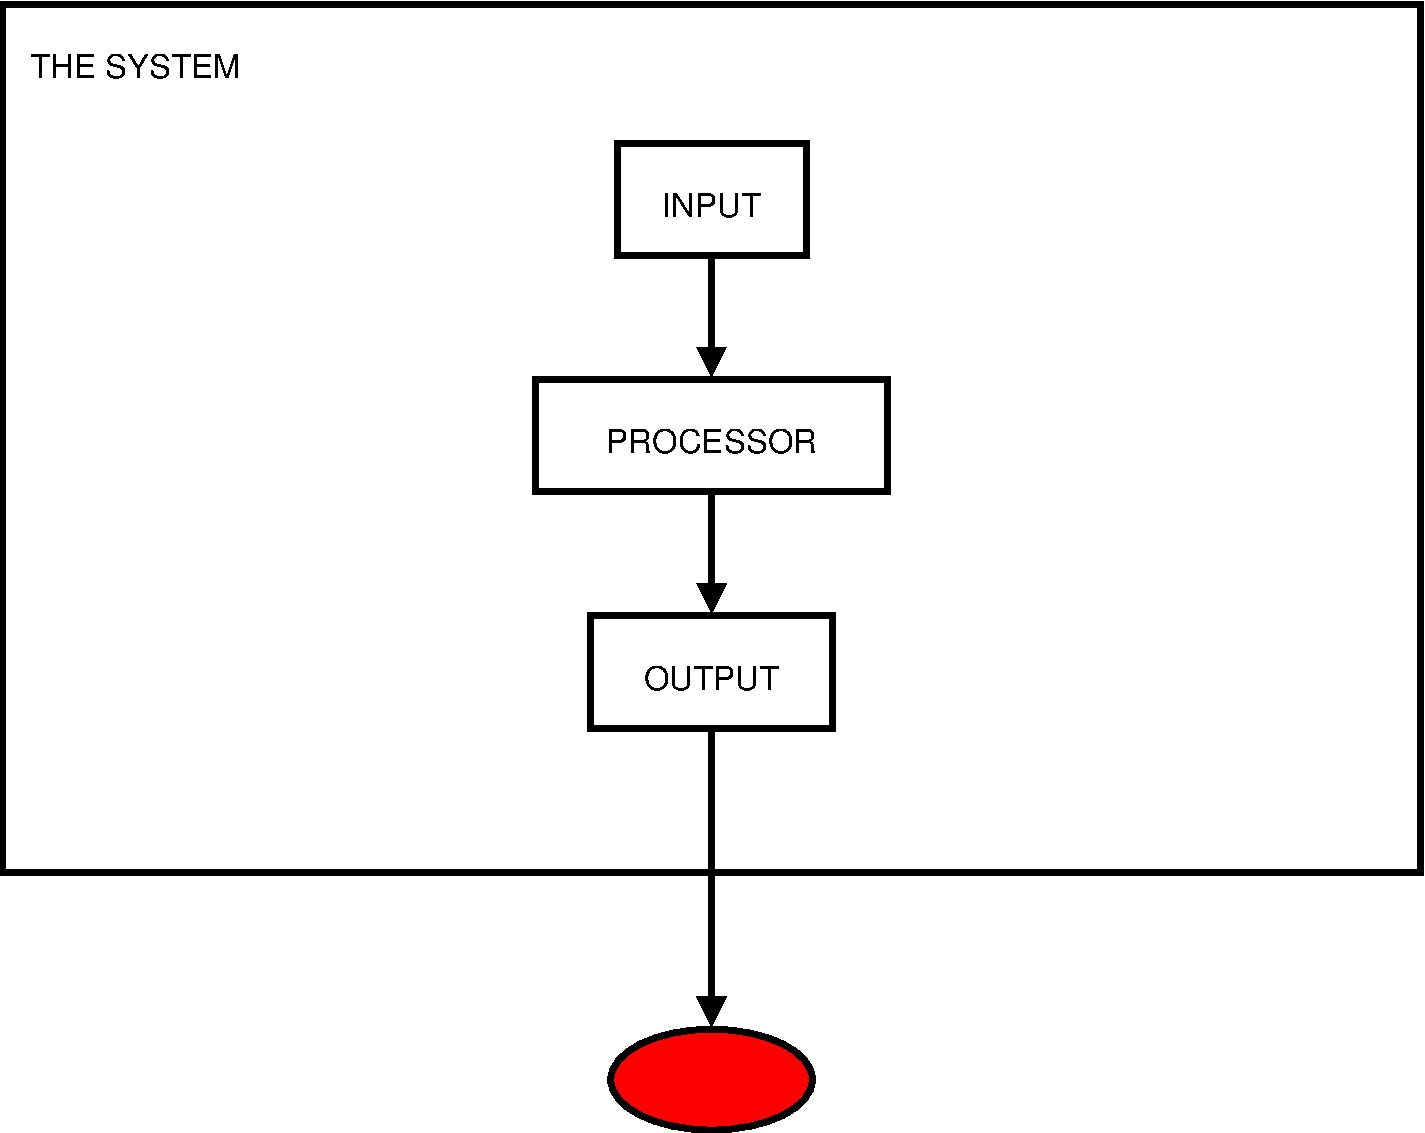
\includegraphics[width=.50\textwidth]{figures/example}
\end{center}
\end{verbatim}
produces the following image:

\need 2 in

\begin{center}
     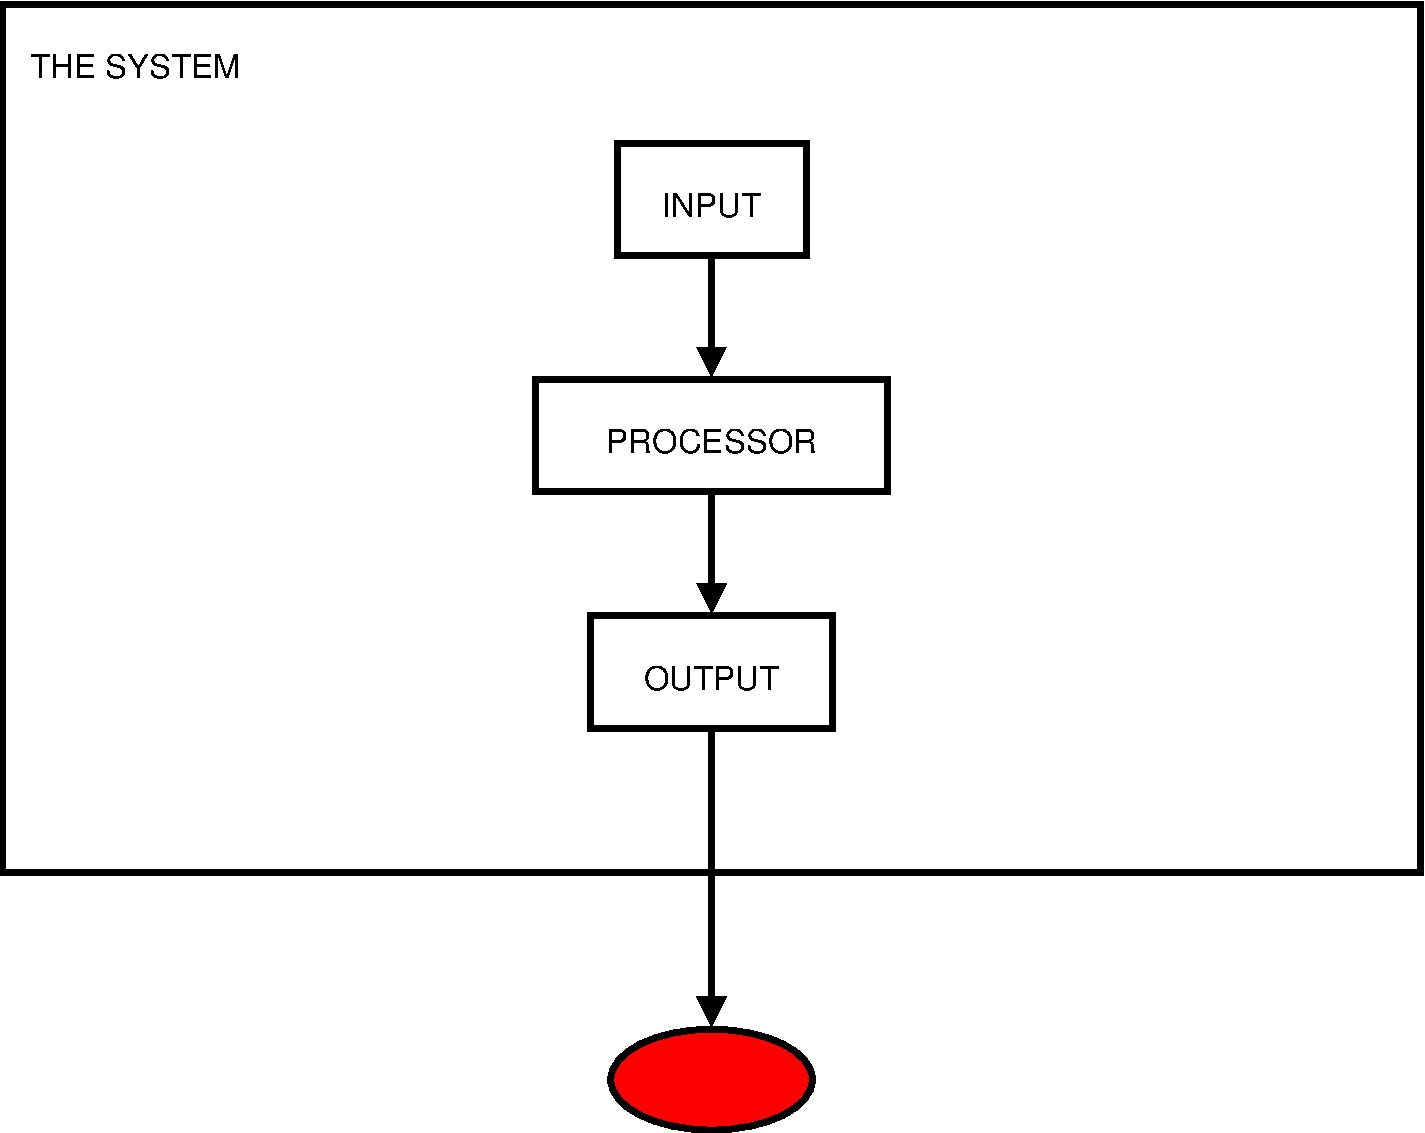
\includegraphics[width=.50\textwidth]{figures/example}
\end{center}

This image looks rather lonely sitting there by itself.  Instructions
for attaching a figure number and a caption to such an image are found
in Chapter~\ref{chap:FIGURESANDTABLES}.

To show you why you should never, ever, ever use a bitmap image if you
have a vector graphics image available, here is an original vector
graphics image and the same image converted to a bitmap.  Need we say more?

\begin{center}
    
\includegraphics[width=.4\textwidth]{figures/oven}
    \quad
    
\includegraphics[width=.4\textwidth]{figures/oven-bitmap}  
\end{center}
%
(OK, one of us can't resist: ``Just don't do it''; ``Friends don't let
friends use bitmap images''; ``Just say no''.  Even if you think your
spreadsheet plot looks good on the screen, do not export it as a
bitmap or use a screen capture program to grab it.)

\subsection {Graphics File Types}

Unfortunately, \LaTeX\ can not use every type of graphics known.
Specifically, \verb|latex| can use encapsulated PostScript
(\verb|.eps|) files, and \verb|pdflatex| can use \verb|.png|,
\verb|.jpg|/\verb|.jpeg| and \verb|.pdf| files.

In the examples above, no file extension was explicitly used, which
means that \verb|latex| or \verb|pdflatex| will pick an appropriate
choice.  How this choice is made is left as a small research project
for the diligent student.

\section {Internal Graphics}

There are two very powerful add-on packages for \TeX\ and \LaTeX: PS
Tricks and TikZ/PGF.  PS Tricks is extremely powerful, but can only be
used (directly) with \verb|latex|; TikZ/PGF is also very powerful, and
can be used with both \verb|latex| and \verb|pdflatex|.

Unfortunately, both of these have a learning curve which is a bit
steep.  However, just to whet your appetite, here are a few
examples using TikZ/PGF.  Note that there are tutorials and
collections of samples to be found on the internet; for example, look
at \url{http://www.texample.net/tikz/examples/}
to see a gallery of sample figures produced using TikZ/PGF. 

Here is a sample of a log-log plot created with the following code:
\begin{verbatim}
  \begin{tikzpicture}
    \loglogaxis
    \addplot coordinates {
        (1,1)
        (16,16)
        (32,64)
    };
    \endloglogaxis
  \end{tikzpicture}
\end{verbatim}

\vspace{10pt}


\pgfplotsset{compat=1.3}% <-- moves axis labels near ticklabels (respects tick label widths)

\begin{tikzpicture}
    \loglogaxis
    \addplot coordinates {
        (1,1)
        (16,16)
        (32,64)
    };
    \endloglogaxis
\end{tikzpicture}

One of the nice things about using TikZ/PGF is that you don't have to
worry about external graphics files becoming separated from the rest of
your document when you move your files from one place to another.

Here is another slightly more complicated example:

\vspace{10pt}

\begin{tikzpicture}
        \loglogaxis[
                xlabel=Cost,
                ylabel=Error]
        \addplot coordinates {
                (5,     8.31160034e-02)
                (17,    2.54685628e-02)
                (49,    7.40715288e-03)
                (129,   2.10192154e-03)
                (321,   5.87352989e-04)
                (769,   1.62269942e-04)
                (1793, 4.44248889e-05)
                (4097, 1.20714122e-05)
                (9217, 3.26101452e-06)
        };
        \addplot coordinates {
                (7,     8.47178381e-02)
                (31,    3.04409349e-02)
                (111,   1.02214539e-02)
                (351,   3.30346265e-03)
                (1023,  1.03886535e-03)
                (2815,  3.19646457e-04)
                (7423,  9.65789766e-05)
                (18943, 2.87339125e-05)
                (47103, 8.43749881e-06)
        };
        \legend{Case 1,Case 2}
        \endloglogaxis
\end{tikzpicture}


The code to produce that is the following:
\begin{verbatim}
  \begin{tikzpicture}
    \loglogaxis[
        xlabel=Cost,
        ylabel=Error]
    \addplot coordinates {
        (5,     8.31160034e-02)
        (17,    2.54685628e-02)
        (49,    7.40715288e-03)
        (129,   2.10192154e-03)
        (321,   5.87352989e-04)
        (769,   1.62269942e-04)
        (1793, 4.44248889e-05)
        (4097, 1.20714122e-05)
        (9217, 3.26101452e-06)
    };
    \addplot coordinates {
        (7,     8.47178381e-02)
        (31,    3.04409349e-02)
        (111,   1.02214539e-02)
        (351,   3.30346265e-03)
        (1023,  1.03886535e-03)
        (2815,  3.19646457e-04)
        (7423,  9.65789766e-05)
        (18943, 2.87339125e-05)
        (47103, 8.43749881e-06)
    };
    \legend{Case 1,Case 2}
    \endloglogaxis
  \end{tikzpicture}
\end{verbatim}

\medskip
As you can see, if you have large amounts of data, you might not want
to massage it into the format required for TikZ/PGF.

Aside from X-Y plots, TikZ/PGF is very nice for creating graphs such
as the following finite automaton:

\usetikzlibrary{automata}
\makeatletter
\def\tikz@double@width@distance{1.6pt}  % default 0.6
\makeatother

\begin{tikzpicture} [shorten >=1pt,>=stealth,node distance=3.5cm,auto]
    %\draw[help lines] (0,0) grid (3,2);
    \node[state,initial,accepting]     (q_0) {$q_0$};
    \node[state]                       (q_1) [right of=q_0] {$q_1$};
    \node[state,accepting]             (q_2) [right of=q_1] {$q_2$};
    \node[state]                       (q_3) [above of=q_1] {$q_3$};
    \path[->]
        (q_0) edge node {0} (q_1)
              edge [loop below] node {1} (q_0)
              edge node {$\epsilon$} (q_3)
        (q_1) edge node {$\epsilon$} (q_2)
              edge [loop below] node {0} (q_1)
        (q_3) edge [loop above] node {0,1} (q_3)
              edge node {1} (q_1);
\end{tikzpicture}


\medskip
That was produced with the following code:

\begin{verbatim}
\usetikzlibrary{automata}
\makeatletter
\def\tikz@double@width@distance{1.6pt}  % default 0.6
\makeatother

\begin{tikzpicture} [shorten >=1pt,>=stealth,node distance=3.5cm,auto]
    %\draw[help lines] (0,0) grid (3,2);
    \node[state,initial,accepting]     (q_0) {$q_0$};
    \node[state]                       (q_1) [right of=q_0] {$q_1$};
    \node[state,accepting]             (q_2) [right of=q_1] {$q_2$};
    \node[state]                       (q_3) [above of=q_1] {$q_3$};
    \path[->]
        (q_0) edge node {0} (q_1)
              edge [loop below] node {1} (q_0)
              edge node {$\epsilon$} (q_3)
        (q_1) edge node {$\epsilon$} (q_2)
              edge [loop below] node {0} (q_1)
        (q_3) edge [loop above] node {0,1} (q_3)
              edge node {1} (q_1);
\end{tikzpicture}
\end{verbatim}

One of the nice things about using a package like TikZ/PGF is that,
while there is a learning curve involved, and there is no
instantaneous visual feedback as when using a programs such as
\verb|xfig|, \verb|dia|, or (*gag*) \verb|visio|, there is also no
endless fussing trying to get the lines and circles arranged in a
visually pleasing, consistent manner.  For example, note that the
edges in the automaton graph all point to the centers of their
corresponding nodes, rather than just pointing to some random spot
on the edge of the node.

A second nice thing about using TikZ/PGF can be observed by reviewing
the figures in Section~\ref{sec:IEG}; the text in these figures does
not match the text in the rest of this chapter (both the typeface and
the size are wrong).  This is a recurring problem when you includes
figures or other graphics created using other programs.  Depending on
the program creating the figure, you may find it either difficult or
impossible to make the text consistent.  When possible, it is nice to
avoid this ugly-ism, and one way to do so is to use TikZ/PGF for your
graphics.

There is a \textbf{very} extensive user manual for this package; on a
Linux system run the command ``\texttt{texdoc tikz}'' to see the
documentation.

As a final example, in Figure~\ref{fig:SNARK} an example of a
(graph-theoretic) graph drawn using TikZ/PGF is shown; note that the
textual labels of the graph perfectly match the rest of the text.  If
you want to see the commands used to create Figure~\ref{fig:SNARK},
look in the \verb|graphics-info.tex| input file.  If you need to
perk your interest a bit more, look at
\url{http://www.texample.net/tikz/examples/} to see a gallery of
sample figures produced using TikZ/PGF.

\begin{figure}[ht]
  \centering
  \begin{tikzpicture}[xscale=1.65,yscale=1.65,thick,
        nodeStyle/.style={shape=circle,minimum size=0.9cm,
            inner sep=0.2pt,draw},
        specialEdge/.style={ultra thick, dashed}]
% For unlabelled small or medium graphs the minimum node size
% looks better at something like 0.3 cm.
    \foreach \num/\theta/\r in {
        1/90/2, 2/18/2, 3/306/2, 4/234/2, 5/162/2}
    {
        \node (\num) at (\theta:\r) [nodeStyle] {$v^{}_{\num}$};
    }
    \foreach \num/\theta/\r/\text in {
            6/90/1/N, 7/18/1/NE, 8/306/1/SE, 9/234/1/SW, 10/162/1/NW}
    {
        \node (\num) at (\theta:\r) [nodeStyle] {\text};
    }
    \path \foreach \u/\v in {
        1/2, 2/3, 3/4, 4/5, 5/1,
        6/8, 7/9, 8/10, 9/6, 10/7, 1/6, 2/7, 3/8, 4/9, 5/10}
    {
        (\u) edge[] node {} (\v)
    };
  \end{tikzpicture}.
  \caption{The Petersen Graph.}
  \label{fig:SNARK}
\end{figure}

Aside from the matching text size and typeface in
Figure~\ref{fig:SNARK}, note the symmetry and precision of the
placement of the circles and the fact that the lines are positioned
exactly as they should be.  Learning a bit of TikZ/PGF to create
figures will take a while, but it is worth it.  (Conversely, doing a
mediocre job with a GUI drawing program is easy, but doing something
worthy of your thesis using most GUI tools is much trickier.)

    %---------------------------------------------------------
% Chapter: A chapter about figures and tables
%----------------------------------------------------------
\chapter{Figures and Tables}
\label{chap:FIGURESANDTABLES}

\section{Floats}

A \emph{float} is an object in a document that should not be broken across
multiple pages. The term ``float'' signifies that \LaTeX\ may move
a floating object within the document to preserve the flow of the
document (e.g., to ensure that the bottom of a page doesn't have a
gaping hole simply because the figure does not fit on the page) and to
improve the alignment of the object if more than one can fit
horizontally on the page.

Understanding what \LaTeX\ will do with a float is important
because the system will make decisions about where to place
a float automatically; the position of the float in your
\emph{source code} may or may not be the same as the position of 
the float in the document.  Learning to trust \LaTeX\ and \TeX\
to do The Right Thing is the first hurdle.

There is much more to know about floats, since packages can
influence their placement. A basic overview along with lots
more information about figures and tables can be found at
\url{http://www.andy-roberts.net/misc/latex/latextutorial6.html},
but to be sure read the documentation for your 
particular package to be sure.

For example, notice below that \LaTeX\ moved Figure~\ref{fig:EXAMPLE1}
and Table~\ref{tab:EQUATION1_VALUES} to follow the paragraph starting
with ``We can also create'', even though the code for those preceded
that paragraph in the \verb|figuresandtables.tex| input file.  That is
because there is not room for them to fit on that page, so
\LaTeX\ ``floats'' them to a future page where there is room to fit
them, without leaving a (possibly) big, sucking, ugly gap at the
bottom of the page.


% This makes a spurious complaint in the log file go away.
\need 2 in

\section{Figures and Tables}

We can use the \verb|figure| environment in order to add a caption and
label to a figure so that it is picked up in the ``List of Figures''.
We can also use the label to reference the figure in the text.  For
example, Figure~\ref{fig:EXAMPLE1} and
Table~\ref{tab:EQUATION1_VALUES} were produced using the commands

\begin{verbatim}
\begin{figure}[ht]
    \centering
    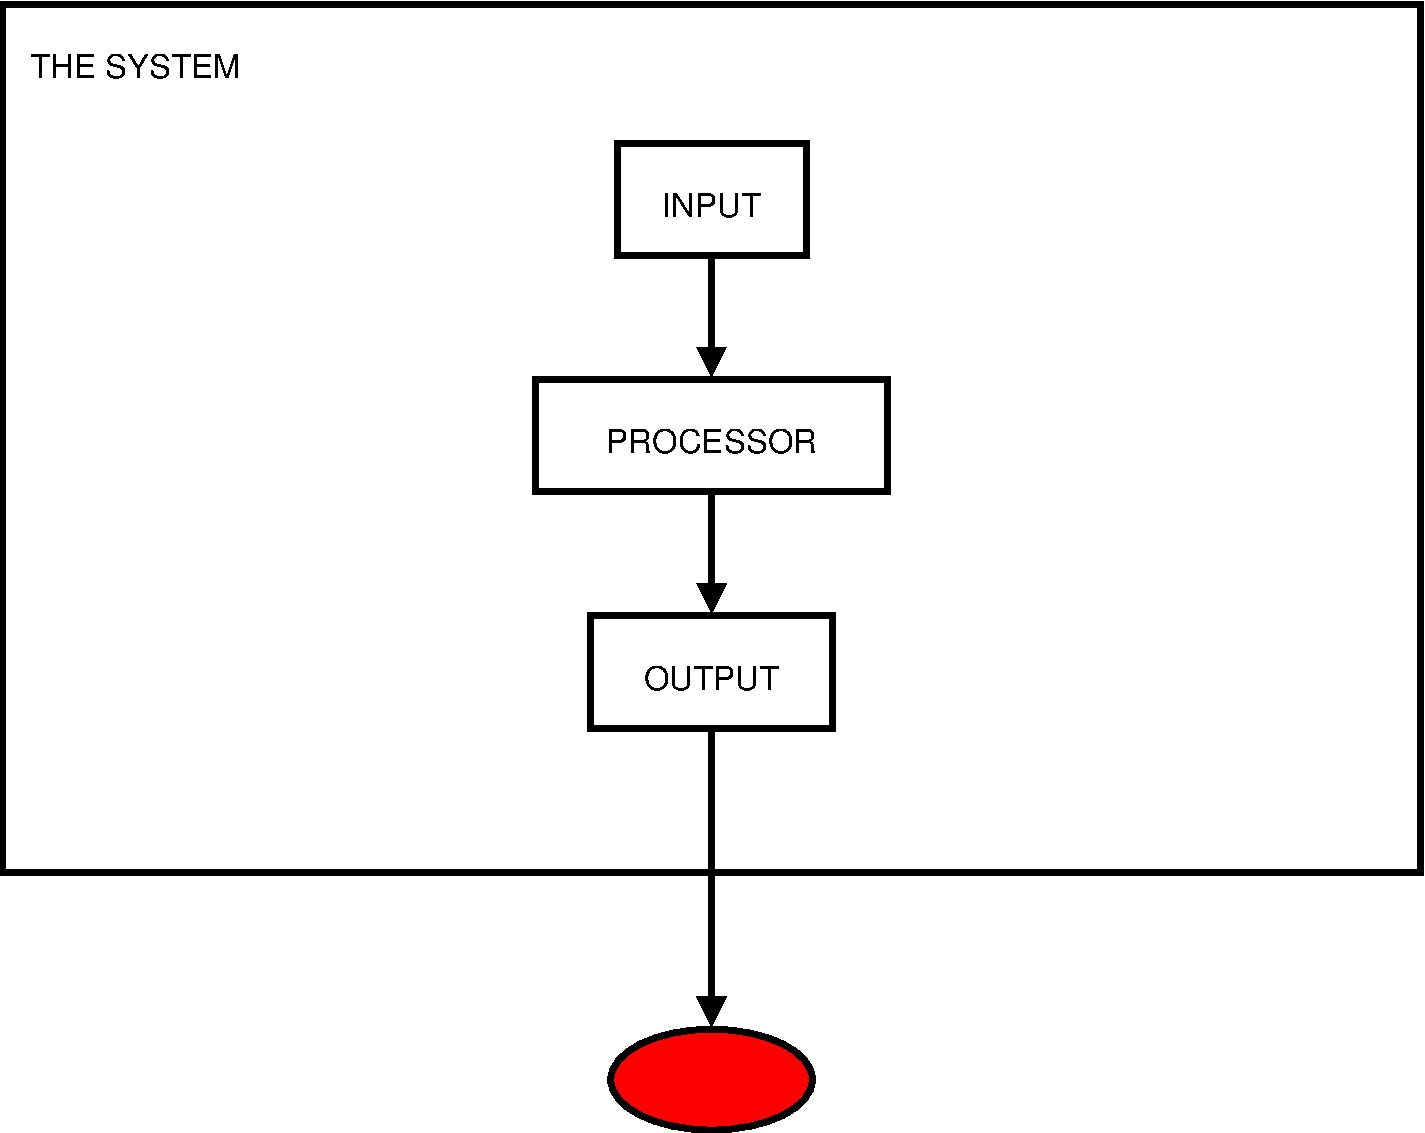
\includegraphics[width=.50\textwidth]{figures/example}
    \caption{An example image.}
    \label{fig:EXAMPLE1}
\end{figure}
\end{verbatim}

\noindent and

\begin{flushleft}
\small
\begin{verbatim}
\begin{table}[ht]
    \centering
    \caption{Table of values for $F(\chi)=\chi+4$.}
    \begin{tabular}[ht]{r|l}
        \hline
        $\chi$ & $F(\chi)=\chi+4$\\
        \hline
        $1$ & $5$\\
        $2$ & $6$\\
        $3$ & $7$\\
        $4$ & $8$\\
        \multicolumn{2}{l}{$\ldots$}\\
        \hline
    \end{tabular}
    \label{tab:EQUATION1_VALUES}.
\end{table}
\end{verbatim}
\end{flushleft}

\begin{figure}[ht]
    \centering
    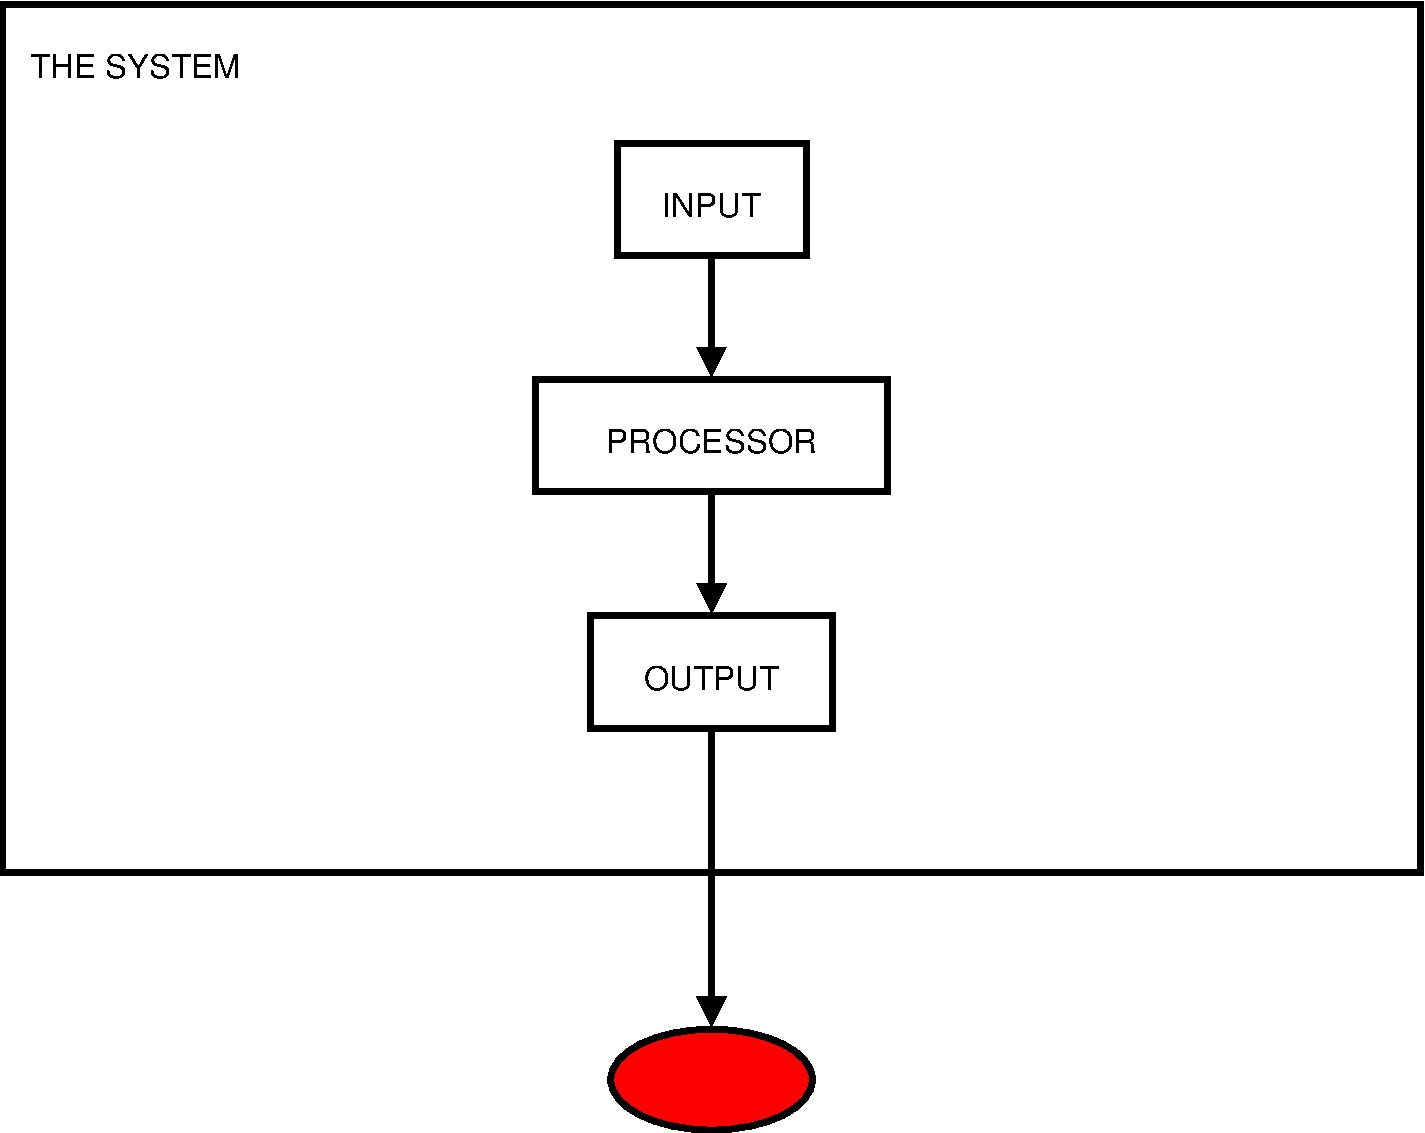
\includegraphics[width=.50\textwidth]{figures/example}
    \caption{An example image.}
    \label{fig:EXAMPLE1}
\end{figure}

\begin{table}[ht]
    \centering
    \caption{Table of values for $F(\chi)=\chi+4$.}
    \begin{tabular}[ht]{r|l}
	\hline
	$\chi$ & $F(\chi)=\chi+4$\\
	\hline
	$1$ & $5$\\
	$2$ & $6$\\
	$3$ & $7$\\
	$4$ & $8$\\
	\multicolumn{2}{l}{$\ldots$}\\
	\hline
    \end{tabular}
    \label{tab:EQUATION1_VALUES}.
\end{table}



We can also create \emph{sub}-figures (Figures~\ref{fig:MIX}
and~\ref{fig:BAKE}) and \emph{sub}-tables (Tables~\ref{tab:SUB1}
and~\ref{tab:SUB2}).  Look at the source for this chapter to see how
it was done, should you want to do it in your thesis.

\begin{figure}[!ht]
    \centering

    \subfloat[Make the Dough]{
    	\label{fig:MIX}
	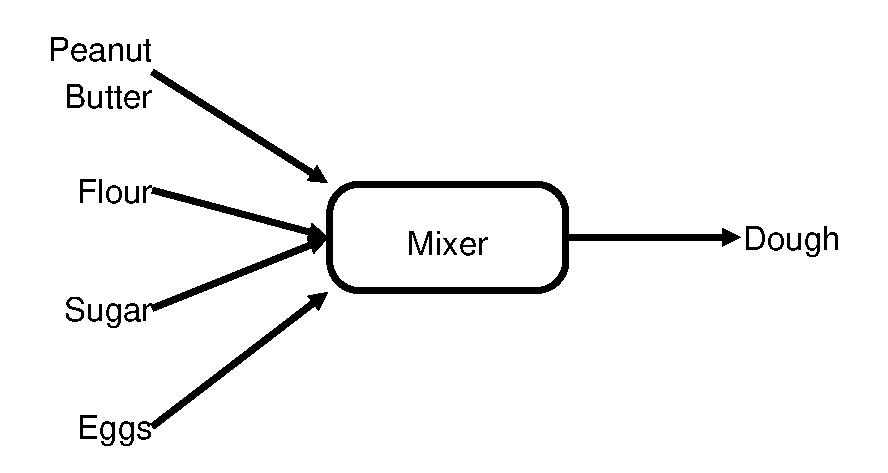
\includegraphics[width=0.45\textwidth]{figures/dough}
    }
     \subfloat[Bake the Cookies]{
    	\label{fig:BAKE}
	
\includegraphics[width=0.45\textwidth]{figures/oven}
    }
    \caption{Making Peanut Butter Cookies.}
    \label{fig:PEANUTBCOOKIES}
\end{figure}

\begin{table}[!ht]
    \centering
    \caption{Table of values for two other $F()$s.}
    \subfloat[$F(z)=x+y$]{
	\label{tab:SUB1}
	\begin{tabular}[ht]{lll}
    	    \hline
    	    $x$ & $y$&$F(z)=x+y$\\
	    \hline
	    $1$ & $2$ & $3$\\
	    $1$ & $3$ & $4$\\
	    $1$ & $4$ & $5$\\
	    $1$ & $5$ & $6$\\
	    $1$ & $6$ & $7$\\
	    \hline
    	\end{tabular}
    }
    \subfloat[$F(z)=x+2y$]{
	\label{tab:SUB2}
    	\begin{tabular}[ht]{lll}
    	    \hline
    	    $x$ & $y$&$F(z)=x+2y$\\
	    \hline
	    $1$ & $2$ & $5$\\
	    $1$ & $3$ & $7$\\
	    $1$ & $4$ & $9$\\
	    $1$ & $5$ & $11$\\
	    $1$ & $6$ & $13$\\
	    \hline
    	\end{tabular}
    }
    \label{tab:EQUATION2_VALUES}.
\end{table}


% This is an ugly way to get the tallstrut defn in the middle of the line.
% Speaking of things not being done the \LaTeX\ way...
% Maybe instead look at the last answer in
% http://tex.stackexchange.com/questions/24186/how-to-center-text-without-adding-space-and-not-altering-alignment-of-surroundin
You may have thought there wasn't enough space above and below the
line with $F(\chi)$ in Table~\ref{tab:EQUATION1_VALUES}.  JD certainly
doesn't think there is enough space there, and he feels that the fact
that \LaTeX's tabular environment doesn't automagically provide enough
space is a bit of a flaw.  JD uses plain \TeX\ rather than \LaTeX, and
thus doesn't know The One True \LaTeX\ Way to fix this, but he would
solve the problem by putting the definition

\begingroup
\leftskip=0cm plus 0.5fil
\rightskip=0cm plus -0.5fil
\parfillskip=0cm plus 1fil
\noindent
\verb|\def\tallstrut{\vrule width 0pt depth 5.5 pt height 12 pt}|
\par
\endgroup
\noindent
before the definition of the table and then changing
``\verb|$\chi$ & $F(\chi)=\chi+4$\\|'' in the table definition to read
``\verb|\tallstrut $\chi$ & $F(\chi)=\chi+4$\\|''.  This produces the
result shown in Table~\ref{tab:EQUATION1a_VALUES}.  The
\verb|depth 5.5pt| and \verb|height 12pt| tell \TeX\ to make sure
there is at least 5.5~pt.\ of space below the typesetting baseline and
12~pt.\ of space above the baseline.  If you decide to go to this
length to make your thesis look good (and why shouldn't you?\null),
keep in mind that you may wish to change these numbers, depending on
what characters are actually used on the line you are prettying up.

\def\tallstrut{\vrule width 0pt depth 5.5 pt height 12 pt}

\begin{table}[ht]
    \centering
    \caption{Table of values for $F(\chi)=\chi+4$.}
    \begin{tabular}[ht]{r|l}
	\hline
	\tallstrut $\chi$ & $F(\chi)=\chi+4$\\
	\hline
	$1$ & $5$\\
	$2$ & $6$\\
	$3$ & $7$\\
	$4$ & $8$\\
	\multicolumn{2}{l}{$\ldots$}\\
	\hline
    \end{tabular}
    \label{tab:EQUATION1a_VALUES}.
\end{table}

Finally, you should note that figures and tables should
\textbf{always} go \textbf{after} the first reference to them in the
text.  The ``\verb|[ht]|'' in the ``\verb|\begin{table}|'' line
indicates that you are happy with the figure going \verb|h|ere or at
the \verb|t|op of a following page.  (You can also use ``\verb|b|''
for the \verb|b|ottom of the page.)
Sometimes \LaTeX\ puts the float further away than necessary; if this
happens to you try changing ``\verb|[ht]|'' to  ``\verb|[!ht]|''. 
If you examine the source code for this chapter you will see this was
done in a couple of places.

    
%---------------------------------------------------------
% Chapter: A chapter about typesetting.  See https://xkcd.com/1015/
%----------------------------------------------------------

\chapter{Some Fine Points of Typesetting}

No-one expects an honours or masters thesis to be a world-class
example of typography (unless, I suppose, you are studying that
discipline).
However, that doesn't mean you shouldn't put a tiny bit more effort in
to make it look as nice as possible.  \TeX\ already takes care of many
of the details for you, but you can help \TeX\ out every now and then.

\section{Non-Breakable Spaces}

In some situations you may want to tell \TeX\ to \emph{not} put a
line-break between two particular words.  For example, you would not
want ``Section'' to be at the end of one line and ``3.2.1'' to be at
the beginning of the next line.  Similarly you don't want ``Figure'',
``Table'', ``Algorithm'', ``Listing'', and so on at the end of one
line and the corresponding number at the beginning of the next line.
(Especially if the next line is at the top of the next page!)

Any time you want to keep to words together, use a ``\verb|~|''
instead of a space between the two words.  For example, earlier you
saw ``\verb|Definition~\ref{def:COOKIE}|''; the ``\verb|~|'' ensures
that the reference number for COOKIE (\ref{def:COOKIE}) does not end
up at the beginning of a line.

To avoid having the last word in a paragraph on a line by itself, but
a \verb|~| between the last two words in the paragraph.  Caution: with
a \textbf{very} short paragraph, this may do more harm than good.  But
you should avoid very short paragraphs anyway (in most situations).

\need 1in

\section{Inter-Sentence Spacing}

In English typography, it is customary to have more space between the
word at the end of a sentence and the word at the beginning of the
next sentence.  Look at the first paragraph in this chapter and you can see
what I mean.   \TeX\ has a heuristic to automagically add this extra space
for you.

Namely, normally a ``\verb|.|'', ``\verb|?|'', or ``\verb|!|'' ends a
sentence when it is followed by white space (or it is at the end of a
line).  However, this rule is not always correct.  For example, in
``I saw H.M.~Schmoe downtown.\null'' the period after ``M'' is not a
sentence-ending period.  \TeX\ assumes this is the case because the
letter before the period is upper-case.

However, sometimes you might end a sentence after an abbreviation:
``Hamiltonian Cycle is in NP.''  To tell \TeX\ that this is a
sentence-ending period, you can separate the upper case letter from
the period as follows: ``\verb|NP\null.|''.

On the other hand, if you say ``My dog's name is Mr.~Smith'' you do
not want \TeX\ to treat ``Mr.\null'' as the end of a sentence.  In
this case if you write ``\verb|Mr.~Smith|'' then \TeX\ will use the
normal amount of inter-word space (and, as a bonus, you won't end up
with ``Mr.\null'' at the end of a line and ``Smith'' at the beginning
of the next line).

\section{Hyphens and Dashes}

There are four separate typographic symbols which you might be tempted
to use the same keyboard character for: ``-'', ``--'', ``---'' and ``$-$''.
The first is a hyphen, used for (wait for it\dots) hyphenated words,
such as ``multi-faceted''.  The second is known as an ``en-dash'', and
should be used when writing a numeric range such as ``40--45''.  The
third is known as an em-dash, and is used --- according to some styles
--- to set off parts of a sentence.  Finally, $-$ is an arithmetic
operator.  These four symbols are obtained with ``\verb|-|'',
``\verb|--|'', ``\verb|---|''and ``\verb|$-$|'', respectively.


\section{Clubs and Widows}


A \emph{widow} is a single line at the top of a page.  A \emph{club}
is a single line at the bottom of a page.  (Other people use different
names, including \emph{orphan}.  Moving on\dots)  I told you that so I
can tell you this.

Widows and clubs are typographically displeasing, and so by default
the \TeX\ typesetting engine has a moderate dislike for widows and
clubs and will try to break paragraphs (when spitting out a page) to
avoid them.  However, if you have lots of figures, tables, listings,
or other such non-textual stuff, or if you like to write short
paragraphs, you may find that \TeX/\LaTeX\ is not able to
automatically avoid them.

This is something you should only worry about when you are very close
to the final copy of your thesis, since minor edits can cause the
content of many following pages to move around.  When you are almost
done, if you want to deal with clubs and widows, read the blurb in
\verb|acadia-hon-thesis.sty| which gives you some information about
going this last typographic mile.

    
%---------------------------------------------------------
% Chapter: A chapter about algorithms
%----------------------------------------------------------

\chapter{Algorithms and Listings}

\section{Algorithms}

Algorithms can be typeset in \LaTeX\ using the \verb|algorithm|
and \verb|algorithmic| packages. Once they have been included
typesetting an algorithm is a snap. For example, the code:

\begin{verbatim}
\begin{algorithmic}[1]        
	\FOR{$i \leftarrow \left[0, 10 \right]$}
	   \PRINT $i$ to the console.
	\ENDFOR
\end{algorithmic}
\end{verbatim}

\noindent produces the output:

\begin{algorithmic}[1]        
	\FOR{$i \leftarrow \left[0, 10 \right]$}
	   \PRINT $i$ to the console.
	\ENDFOR
\end{algorithmic}

In this example the \verb|[1]| argument to the algorithmic 
environment tells the package to place Arabic numbers at
the beginning of each line.

Like figures and tables, algorithms can be labelled and
captioned.  For example, the code:

% Start a new page if there is less than one inch remaining here:
\need 1 in

\verbatiminput{./algorithms/examplealg}
	
\noindent produces the following typeset algorithm, which can 
be referenced as Algorithm~\ref{alg:EXAMPLE_ALG} by typing
\verb|Algorithm~\ref{alg:EXAMPLE_ALG}|:
	
%------------------------------------------
% Algorithm: Packet size : PACKETSIZE_ALG
%------------------------------------------
\begin{algorithm}[h]
    \centering
    \small
    \caption{Prints out each odd number from $0\rightarrow n-1$ in
	unary, and $n$ in decimal.} 
    \begin{algorithmic}[1]
        \REQUIRE
	    $n$, an integer number where $n \geq 1$
	\ENSURE
	    Prints out each odd number from $0 \rightarrow n-1$ in unary.\\
	    Prints out $n$ in decimal.
	\FOR{$i \leftarrow \left[0, n \right]$}
	    \IF{$i = n$}
		\PRINT Emit $i$ to the stream.
	    \ELSIF{$i \% 2 != 0$}
		\STATE
		    \COMMENT{Then $i$ is odd.}
		\STATE
		     $j \leftarrow i$
		\WHILE{$j \geq 0$}
		    \STATE
		    Emit $1$ to the stream.
		    \STATE
		    $j \leftarrow j - 1$
		\ENDWHILE				
	    \ELSE[Then $i$ is even.]
		\STATE
		\COMMENT{Print nothing!}
	    \ENDIF
	\ENDFOR
    \end{algorithmic}
    \label{alg:EXAMPLE_ALG}
\end{algorithm}


\section{Listings}

Listings in \LaTeX\ can be typeset using the \verb|listings|
package.  We can include code within the text using:

\begin{verbatim}
\begin{centering}
\lstinputlisting[float=h,language=FILE_LANGUAGE,
                 caption=A CAPTION,label=THE_LABEL]{FILE_TO_LIST}
\end{centering}
\end{verbatim}

For example, to include a centered listing of the contents of the 
Java file located at \verb|./examples/example.java|, with a 
caption ``Example Java File.'' and a label \verb|lst:JAVA|, 
we would write:

\begin{verbatim}
\begin{centering}
    \lstinputlisting[float=h,language=Java,caption=Example Java File.,
                     label=lst:JAVA]{./examples/example.java}
\end{centering}
\end{verbatim}

\noindent which would produce Listing~\ref{lst:JAVA}.

\begin{centering}
    \lstinputlisting[float=h,language=Java,caption=Example Java File.,
                     label=lst:JAVA]{./examples/example.java}
\end{centering}

\noindent
But what if we only want to show a few of the lines of the Java program?

In this case we can tell the package to only include certain lines, for
example, lines $10 \rightarrow 11$ in file \verb|./examples/example.java|
would be written

\begin{verbatim}
\begin{centering}
    \lstinputlisting[float=h,firstline=10,lastline=11,language=Java,
        caption=Partial Java Listing.,
        label=lst:SOMEJAVA]{./examples/example.java} 
\end{centering}
\end{verbatim}

\noindent and would produce Listing~\ref{lst:SOMEJAVA}.

\begin{centering}
    \lstinputlisting[float=h,firstline=10,lastline=11,language=Java,
	caption=Partial Java Listing.,
	label=lst:SOMEJAVA]{./examples/example.java} 
\end{centering}

The \verb|listings| package is capable to working with a large number
of languages; you can find the documentation at: 
	\url{http://www.ctan.org/tex-archive/macros/latex/contrib/listings/listings-1.3.pdf}.


For example, to typeset an XML file using a ``footnote-sized'' font we would
use the code:
\begin{verbatim}
\begin{centering}
    \lstinputlisting[float=h,basicstyle=\footnotesize,language=XML,
        caption=Example XML File.,
        label=lst:XML]{./examples/simple_example_xml.xml}
\end{centering}
\end{verbatim}

\noindent which would produce Listing~\ref{lst:XML}.

\begin{centering}
    \lstinputlisting[float=h,basicstyle=\footnotesize,language=XML,
        caption=Example XML File.,
        label=lst:XML]{./examples/simple_example_xml.xml}
\end{centering}

% Defunct link... what did Brian mean by ``sizes'' anyway?
%For more information on sizes see:
%\url{http://www.eng.cam.ac.uk/help/tpl/textprocessing/teTeX/latex/latex2e-html/ltx-178.html}.



    %---------------------------------------------------------
% Chapter: A chapter about packages
%----------------------------------------------------------
\chapter{Packages}

You might find some or all of the following packages useful for
writing your thesis.  To find out more options about these packages,
you can read the corresponding manual.  On a Linux system you should be
able to read (for example) the hyperref documentation by executing the
command \verb|texdoc hyperref|.


\begin{description}
    \item[textcomp] Useful for some extra symbols.
    \item[inputenc] Specifies the encoding format of inputs.
      Generally you would use \verb|latin1| for a thesis written in
      English.
    \item[amsmath] Many useful math mode bits. 
    \item[amsfonts] Fonts for use in math mode (e.g., subscript sized
    Greek letters). 
    \item[amssymb] Extra math symbols (not necessarily useful).
    \item[amsth] Allows you to define ``theorem-like'' sections
    (e.g., the definition used earlier).
    \item[graphicx] Package for graphics functionality and quality.
    \item[soul] Provides ability to ``\textbf{s}trike \textbf{o}ut''
      and \textbf{u}nder\textbf{l}ine text (e.g., useful at
    editing time).
    \item[hyperref] Provides hyper-linking within the PDF output file.
    % If
    % used with the \verb|linktocpage| option the page numbers in
    % the table of contents are hyperlinks to the corresponding pages.
      At time of writing, the options given to the hyperref package in
      this sample thesis' \verb|header.tex| cause the table of
      contents entries, figure and tables numbers, bibliographic
      references and various other things to be hyperlinks.  That is,
      if you see (for example) ``Figure~\ref{fig:EXAMPLE1}'' and you
      click on the ``\ref{fig:EXAMPLE1}'', your PDF viewer should take
      you to that figure.  (Try it out right now.)
      Note that in \verb|header.tex| there are a few fields you should
      edit by hand to register the author and title of your thesis
      inside the PDF file.
    \item[listings] A very powerful listings package to make life easier.
    \item[subfig] Allows you to create sub-figures and subtables (using
    \verb|\subfloat|) within figures and tables.  This replaces the old
    \verb|subfigure| package which is deprecated.
    \item[verbatim] Allows for the use of the \verb|verbatim| environment
    which makes it easier to include multi-line text verbatim in the
    document.
    \item[alltt] Allows for including text that is typed in typewriter
    font. The text is interpreted as code, so be careful of the \TeX\ and 
    \LaTeX\ commands you use.
    \item[natbib] Better control over your bibliography, including
    citation style within the document (e.g., saying \citet{1188581}
    versus just \citep{1188581}).  Numerous customization parameters. 
    \item[acadia-hon-thesis] The ``hopefully-done (for 2015/16,
      anyway)'' Acadia honours style package which was used for this
      sample thesis.
    \item[algorithm] Adds powerful/clean algorithm functionality. 
    \item[algorithmic] Adds an algorithmic environment to your
    documents.  Allows for labeling, captioning, etc.
    \item[tikz] This is a very powerful package for producing many
    different kinds of plots, diagrams, graphs, and so on.  Including
    this package gives you the basic capability; to get additional
    capabilities you need additional \verb|\usepackage| commands (put
    them in \verb|header.tex|).  For example, the data plots shown in
    Chapter~\ref{chap:GRAPHICS} require the use of
    \verb|\usepackage{pgfplots}|.
\end{description}

    % APPENDICES
    \appendix
    \chapter{Web sites}
\label{chap:websites}

Here are a few web sites that you may find useful.  Note that these
links are all ``click-able'' from a PDF file because they were entered with
the ``\verb|\url{...}|'' command.  There is also the
``\verb|\href{mylink}{mytext}|'' command, which creates a link to
\verb|mylink|, but puts the \verb|mytext| as the visible text in your
document.

\begin{itemize}
    \item \url{http://www.google.com}.  (Duh.)
    \item \TeX{}live: \url{http://tug.org/texlive/}.
	One of the free \TeX\ systems, and maybe the best.
    \item Citations Site: \url{http://merkel.zoneo.net/Latex/natbib.php}.
    \item CTAN (the Comprehensive \TeX\ Archive Network):
	\url{http://www.ctan.org/}.  This site contains most
	freely-available \TeX\ resources (including \LaTeX\ itself and
	many contributed packages).
    \item A FAQ: \url{http://www.tex.ac.uk/cgi-bin/texfaq2html}.
    \item MiKTeX: \url{http://www.miktex.org/}.
    \item Many Tikz and PGF graphics examples:
	\url{http://www.texample.net/}.
	If you want to use PGF/TikZ, this is a good place to look for
	a plot, picture, graph or diagram similar to the one you want.
	You can peruse the output images and then download the
	corresponding source code.
    \item Some symbols: \url{http://www.agu.org/symbols.html}.
\end{itemize}


    % \include{an_APPENDIX}
    % \include{another_APPENDIX}
    % CHAPTER CONTENT END

    \bibliography{thesisbib}
\end{document}
